\documentclass[12pt,a4paper,fontset=none]{ctexart}

\usepackage[a4paper,margin=2.54cm]{geometry}
\usepackage{setspace}
\usepackage{array}
\usepackage{booktabs}
\usepackage{tabularx}
\usepackage{graphicx}
\usepackage{float}
\usepackage{xcolor}
\usepackage{hyperref}
\usepackage{listings}
\usepackage{caption}
\usepackage{enumitem}
\usepackage{fancyhdr}
\usepackage{amsmath}
\usepackage{amssymb}
\usepackage{titlesec}
\usepackage{algorithm}
\usepackage{algpseudocode}
\setCJKmainfont[BoldFont={Heiti SC}]{STSong}
\setCJKsansfont{Heiti SC}
\setCJKmonofont{Heiti SC}
\setCJKfamilyfont{zhsong}{STSong}
\setCJKfamilyfont{zhhei}{Heiti SC}
\setCJKfamilyfont{zhkai}[Path={/System/Library/AssetsV2/com_apple_MobileAsset_Font8/88d6cc32a907955efa1d014207889413890573be.asset/AssetData/},FontIndex=0]{Kaiti.ttc}
\ctexset{
  today=big,
  section={
    format+=\bfseries
  },
  subsection={
    format+=\bfseries
  }
}

\hypersetup{
  colorlinks=true,
  linkcolor=black,
  urlcolor=blue,
  citecolor=black
}

\setstretch{1.35}
\setlength{\parindent}{2em}
\setlength{\parskip}{0.3em}
\emergencystretch=2em
\setlength{\headheight}{15pt}

\pagestyle{fancy}
\fancyhf{}
\fancyfoot[C]{\thepage}

\titleformat{\section}{\zihao{4}\bfseries}{\thesection}{0.8em}{}
\titleformat{\subsection}{\zihao{-4}\bfseries}{\thesubsection}{0.8em}{}
\titleformat{\subsubsection}{\normalsize\bfseries}{\thesubsubsection}{0.8em}{}

\lstset{
  basicstyle=\ttfamily\small,
  breaklines=true,
  frame=single,
  columns=fullflexible,
  backgroundcolor=\color{gray!5},
  keywordstyle=\color{blue!70!black},
  commentstyle=\color{green!40!black},
  stringstyle=\color{red!60!black},
  showstringspaces=false
}
\lstdefinelanguage{json}{
  morestring=[b]",
  stringstyle=\color{red!60!black},
  morecomment=[l]{//},
  commentstyle=\color{green!40!black}
}

\begin{document}

\begin{titlepage}
  \centering
  \vspace*{5.8cm}

  {\fontsize{30pt}{48pt}\selectfont 本地 Web 安全配置缺陷与}\\[0.8cm]
  {\fontsize{30pt}{48pt}\selectfont TLS 证书可信性风险检测研究}\\[2.8cm]

  \renewcommand{\arraystretch}{1.75}
  \begin{tabular}{>{\raggedleft\arraybackslash}p{3.0cm}@{\hspace{1.2cm}}>{\raggedright\arraybackslash}p{5.8cm}}
    课程名称： & 网络信息安全风险技术编程 \\
    姓\hspace{1.65em}名： & 寇得一 \\
    学\hspace{1.65em}号： & 2023211545 \\
    班\hspace{1.65em}级： & 2023211801 \\
    指导教师： & 昌硕 \\
  \end{tabular}

  \vfill
  {\zihao{3}2026 年 5 月 20 日}
\end{titlepage}

\pagenumbering{Roman}

\begin{center}
  {\zihao{3}\CJKfamily{zhkai}\bfseries 摘要}
\end{center}

{\CJKfamily{zhkai}
随着网络服务规模的扩大和应用部署频率的提升，由基础安全配置疏漏引发的风险问题日益突出。开放测试端口、目录索引暴露、HTTP 安全响应头缺失、服务版本信息泄露以及 HTTPS 配置不规范等问题，虽然未必直接构成高复杂度漏洞，却往往是攻击者开展信息收集、漏洞匹配和定向攻击的前提条件。针对这一类高频、低门槛且易被忽视的安全隐患，本文设计并实现了一套本地网络资产与 Web 安全配置风险检测系统。系统以 Python 为实现语言，采用“端口探测、协议分析、规则评分、报告生成”的整体思路，能够对目标主机开放端口、HTTP 安全头、目录浏览暴露、服务版本信息以及 HTTPS 基础安全状态进行自动化检测，并输出结构化结果和面向文档展示的风险报告。

在实验部分，本文构建了本地弱安全配置演示环境，并以 \texttt{127.0.0.1} 为目标执行扫描。基础实验结果表明，系统成功识别出 8080 测试端口暴露、目录索引暴露、Server 版本信息泄露以及多项安全响应头缺失等典型问题，综合风险评分为 76，整体等级判定为中风险。在此基础上，本文进一步搭建了基于本地自签名证书的 HTTPS 演示服务，对系统的 TLS 检测模块进行了专项验证，真实复现了证书不受信任（自签名）这一常见 HTTPS 配置风险，使代码实现、执行结果与风险展示三个环节实现了完整闭环。为进一步说明系统定位，本文还从端口检测、HTTP 安全头检测、风险评分、整改建议和代码透明性等维度，将本系统与 Nmap、Nessus、OWASP ZAP、nikto 等主流安全扫描工具进行对比，突出该系统在轻量化实现、低依赖运行和可解释输出方面的差异化价值。同时，为保证代码实现、实验输出与报告材料能够统一查阅和复现，本文已将项目整理并推送至 GitHub 仓库 \href{https://github.com/AndrewAccuracy/WebTLSRiskInspector}{AndrewAccuracy/WebTLSRiskInspector}。

\noindent 关键词：网络信息安全；风险检测；Web 安全配置；端口扫描；自动化巡检
}

\newpage
\tableofcontents
\newpage
\pagenumbering{arabic}

\section{引言}

\subsection{研究背景}

在当前网络空间环境中，传统“边界清晰、业务稳定”的信息系统形态正在被“服务快速上线、环境持续迭代、组件高度复用”的建设模式所替代。云计算、虚拟化、容器编排以及持续集成持续交付技术的普及，使信息系统的部署和变更效率大幅提升，但与此同时，也使系统的攻击面管理问题变得更为复杂 \cite{nist,nist-vuln,nist-csf,owasp-top10}。对于安全管理者而言，风险不再只来自少量高危漏洞本身，还来自海量基础配置项在长时间运行过程中的漂移、遗留和失控。

从实践角度看，许多真实安全事件并不是由高级攻击技术直接触发，而是以信息收集和低成本探测为起点。攻击者往往首先确认目标系统的开放端口、服务类型、目录结构、组件版本以及浏览器侧保护机制是否存在缺口 \cite{wstg,nessus-guide,nmap-book,shodan}。在这一过程中，目录索引暴露、测试端口遗留、默认页面未清理、证书过期、HTTP 安全头缺失等问题常常成为构造后续攻击链的突破口。这类风险虽然在单独出现时不一定立即造成严重后果，但一旦与组件漏洞、弱口令、权限配置错误或运维疏漏叠加，就可能迅速演化为数据泄露、横向移动或业务中断事件 \cite{nist-server,owasp-asvs,cis-controls,mitre-attck}.

更重要的是，基础安全配置问题具有高度的“日常性”。与漏洞利用往往依赖特定条件不同，配置问题普遍存在于服务上线、环境迁移、系统扩容和运维交接等普通流程中。它们的出现不一定源于开发人员缺乏安全意识，很多时候只是由于业务上线节奏过快、检查流程未固化、责任边界不清晰或者安全基线缺少自动校验机制所造成 \cite{devsecops,ssdlc,secure-by-design,nist-scrm}。因此，针对这类问题建立自动化、可复用、可解释的检测机制，能够将分散的配置状态转化为可审计的风险证据，也能够为后续处置提供相对稳定的判断依据。

这类风险还呈现出三个显著特征。其一，发现成本低，攻击者通常无需投入过高技术门槛即可完成识别；其二，影响链条长，一个看似普通的配置疏漏可能成为后续漏洞利用、越权访问乃至数据泄露的起点；其三，治理依赖持续巡检，仅靠上线前的一次性人工检查往往难以覆盖长期运行过程中的配置漂移 \cite{owasp-cheatsheet,nist-80053,cis-benchmarks,ops-report}。因此，将基础安全配置风险转化为程序可识别、可度量、可输出的自动化检测对象，具有明确的现实价值。

\subsection{研究目的与意义}

本文的目标是设计并实现一个面向本地网络资产与 Web 服务配置状态的轻量级风险检测系统，并将“风险可见、风险可测、风险可解释”作为系统建设的核心标准。所谓“可见”，是指风险能够通过程序结果被明确列举和描述；所谓“可测”，是指风险项能够借助评分机制进行量化；所谓“可解释”，是指检测结果能够以证据、规则和整改建议的形式说明判定依据。换言之，本文不仅追求“扫描到问题”，更强调“解释问题、比较问题和展示问题”。

本研究的意义主要体现在以下三个方面。第一，从方法层面看，本文尝试将基础安全巡检任务拆解为端口探测、协议访问、规则映射和量化输出四个可编程阶段，展示如何将经验性的安全检查动作转化为程序逻辑 \cite{owasp-asvs,websec-book,practical-monitoring}。第二，从实现层面看，本文以自研程序完成关键检测流程，避免将风险识别过程完全交给封闭工具，从而使端口状态、响应头特征、目录索引证据和评分规则都能够被逐步追踪。第三，从工程层面看，该系统具备一定扩展潜力，可进一步演进为持续巡检、批量主机检测、风险台账生成或可视化安全基线工具的原型 \cite{nuclei,openvas,devsecops,security-automation}。

此外，本文特别关注“轻量级实现”的价值。现实中的安全产品往往功能完善、规则丰富，但在分析一个具体检测系统时，如果完全依赖成熟工具，容易削弱对检测逻辑本身的展开。相比之下，基于标准库构建的小型检测系统更有助于呈现核心逻辑、说明设计取舍，并使读者清楚地理解每一项风险是如何被发现、归类和评分的 \cite{software-security,secure-coding,threat-modeling}。

\subsection{研究内容}

围绕上述目标，本文的主要工作包括：

\begin{enumerate}[label=\arabic*.]
  \item 分析本地网络资产与 Web 基础配置中的典型风险点；
  \item 设计端口探测、HTTP/HTTPS 检测、规则评分与报告生成的系统架构；
  \item 使用 Python 标准库完成核心检测逻辑开发；
  \item 构建弱安全配置演示环境，验证系统对典型风险的识别能力；
  \item 对实验结果进行分析，并提出相应的预防与改进措施。
\end{enumerate}

\subsection{论文结构安排}

为便于系统性展示研究思路与实现过程，本文后续内容按如下结构展开：第二章对基础安全配置风险的典型表现、研究任务边界与系统需求进行分析；第三章给出系统总体设计思路、模块划分和风险评分模型；第四章介绍系统的关键实现方法与算法逻辑；第五章展示实验过程与执行结果；第六章对风险含义、量化结果和方法局限进行讨论；第七章提出预防措施与改进建议；最后对全文工作进行总结。这样的结构安排能够将“问题提出一系统设计一实验验证一结果讨论”完整串联起来，使本文围绕同一检测对象形成闭环论证。

\section{相关问题分析与需求定义}

\subsection{基础安全配置风险的典型表现}

在网络与应用系统中，基础安全配置风险的外在表现非常丰富，但从检测视角出发，可以大致归纳为“暴露面风险、协议配置风险、信息泄露风险和加密通信风险”四类 \cite{owasp-top10,wstg,nist-server,cis-benchmarks}。这四类问题之间既相互独立，又彼此联系，共同构成了系统在日常运行中的基础安全状态。

第一类是暴露面风险，即系统对外开放了不必要的网络入口，或者虽然开放了端口，但缺乏相应的访问控制与用途约束。典型情形包括测试服务遗留在线、后台管理端口未限制来源地址、数据库端口误暴露、缓存或中间件服务直接对公网可见等 \cite{shodan,redis-security,mysql-security,nmap-book}。这类问题的危险性在于，它们并不一定直接构成漏洞，但会极大提升攻击者开展侦察和攻击尝试的机会。

第二类是协议配置风险，主要体现在 HTTP 与 HTTPS 的防护机制未按安全基线落实。HTTP 响应头本身是协议语义的标准组成部分 \cite{rfc9110}，例如，站点缺少 HSTS、CSP、X-Frame-Options、X-Content-Type-Options 和 Referrer-Policy 等安全响应头时，浏览器侧将缺乏足够的约束和保护能力 \cite{rfc6797,csp,xcto,referrer-policy,clickjacking}。又如，TLS 版本仍停留在 1.0 或 1.1，或者保留弱密码套件，也会使加密通信的安全强度下降 \cite{rfc8446,tls-bcp,mozilla-tls,owasp-tls}。

第三类是信息泄露风险，即系统无意中向外界暴露了本不应公开的环境信息、软件信息或资源结构信息。常见表现包括 \texttt{Server} 头暴露精确版本号、默认错误页泄露中间件信息、目录索引暴露资源层次、调试页面保留在生产环境以及备份文件、日志文件等可被直接访问 \cite{wstg,owasp-cheatsheet,apache-security,nginx-security}。这些信息单独来看可能只是“细节”，但对攻击者而言却往往是极具价值的情报来源。

第四类是加密通信风险，主要围绕证书管理、协议协商与通信完整性展开。证书过期、证书链配置不完整、启用不再推荐的协议版本、支持弱加密套件等问题，都会削弱系统对中间人攻击和流量分析的抵御能力 \cite{rfc8446,tls-bcp,nist-crypto,cert-guide}。在许多组织中，这类问题的根源并不在于技术实现本身，而在于证书更新流程缺乏持续监控，或者系统历史兼容性包袱较重。

这些问题虽然类型不同，但都具有较强的可检测性，适合通过程序规则化表达。一方面，它们大多可以通过网络交互直接观测到；另一方面，它们的判定条件相对清晰，便于通过布尔规则、阈值规则和特征匹配规则进行编码。也正因如此，它们适合作为本文检测系统的核心风险对象。

\subsection{研究任务边界}

本文围绕网络信息安全风险技术中的基础配置风险展开，重点体现“自主开发”而非“直接使用现成安全产品”。这意味着系统不能只是调用成熟工具输出结果，而应当在核心检测逻辑、规则组织方式和结果呈现机制上体现清晰的编程设计思路。换言之，本文关注的重点不仅在于“最终有没有扫出问题”，更在于“问题是如何被程序发现、解释并组织成报告的”。

围绕上述研究任务，系统在设计时必须兼顾以下要求：

\begin{enumerate}[label=\arabic*.]
  \item 主要检测逻辑由本人编写完成；
  \item 结果应具备清晰的结构化表达形式；
  \item 风险输出不仅要指出问题，还应能够解释问题；
  \item 整体材料应能自然组织成论文式报告。
\end{enumerate}

此外，本文还设定两个边界条件。其一，系统应具有可复现性，即在本地环境中能够构建稳定的弱配置场景，并重复得到一致的检测结果；其二，系统应具有可扩展性，即当前实现虽然只覆盖基础风险，但架构上应为后续追加规则、扩展目标范围和增强展示方式留有空间。正是在这些约束下，本文选择了“本地网络资产与 Web 安全配置风险检测”这一兼顾可操作性与现实性的研究方向。

\subsection{功能需求}

基于上述分析，本文将系统功能需求定义如下。需要说明的是，这些需求并非简单罗列，而是与整体检测流程一一对应。前两项需求对应“目标发现”，中间三项需求对应“风险识别”，最后两项需求则服务于“结果表达与分析”。

\begin{enumerate}[label=\arabic*.]
  \item 对指定主机的多个端口执行连通性检测；
  \item 对开放端口进行服务类型映射，并给出基础暴露风险提示；
  \item 对 HTTP 服务执行响应头获取和正文预览；
  \item 检测目录索引暴露、版本信息泄露和安全响应头缺失等问题；
  \item 对 HTTPS 服务执行证书和 TLS 基础安全检测；
  \item 基于规则模型计算风险总分和总体等级；
  \item 自动生成 JSON 与 Markdown 报告文件。
\end{enumerate}

进一步细化来看，这些功能需求可以分为“检测型需求”和“表达型需求”两类。检测型需求关注系统能否正确收集与判定风险事实，例如端口是否开放、响应头是否缺失、证书是否过期；表达型需求则关注系统能否将这些事实转化为易于理解和使用的结果，例如是否能够给出证据、建议、风险等级和综合评分。对于本文而言，后者同样重要，因为它决定了系统是否真正实现了“风险可见、可测、可解释”。

\subsection{非功能需求}

除功能需求外，系统还需满足如下非功能要求：

\begin{enumerate}[label=\arabic*.]
  \item 轻量性：尽量依赖标准库，降低部署和运行成本；
  \item 可解释性：每个风险项需附带证据和整改建议；
  \item 可扩展性：便于后续增加新的检测规则与输出形式；
  \item 可复现性：实验环境应可在本地快速搭建并重复执行。
\end{enumerate}

其中，“轻量性”和“可复现性”是本文特别强调的两个属性。基础风险检测系统若强依赖复杂外部环境，往往会增加部署、复测和结果解释的成本。采用标准库与本地演示环境相结合的方式，既能降低运行门槛，也便于重复验证结果。与此同时，“可解释性”与“可扩展性”则直接决定了系统是否具备从本地原型进一步走向工程化雏形的潜力 \cite{software-engineering,monitoring-book,secure-design,platform-engineering}。

\subsection{需求与设计之间的映射关系}

为了避免需求分析与系统设计相互脱节，本文进一步将关键需求与后续模块设计建立映射关系。端口连通性检测需求对应端口扫描模块，HTTP/HTTPS 配置检查需求对应协议分析模块，风险评分需求对应规则评分模块，报告输出需求对应结果生成模块。通过这种映射，可以保证系统设计并非从抽象架构出发，而是直接服务于前文定义的需求集合。

这种“需求一模块一结果”的映射关系还有一个额外好处，即便于后续验证系统是否真正实现了预期目标。例如，当实验中成功识别出目录索引暴露和安全头缺失时，就可以回溯到对应的功能需求与模块逻辑，证明系统不仅“运行成功”，而且“实现闭环”。这也使本文的实验结果能够直接支撑前文提出的系统目标。

\section{系统设计}

\subsection{总体设计思路}

本文提出的检测系统采用“探测一分析一评分一输出”的流水线式处理思路。系统首先从网络层识别目标暴露面，随后在协议层采集 HTTP 或 HTTPS 的运行特征，再利用规则引擎对采集结果进行语义化解释，最后将风险项汇总为结构化报告和文本报告。该思路既保留了实现上的简洁性，又较好地体现了风险分析的层次性与可解释性。

\begin{figure}[H]
  \centering
  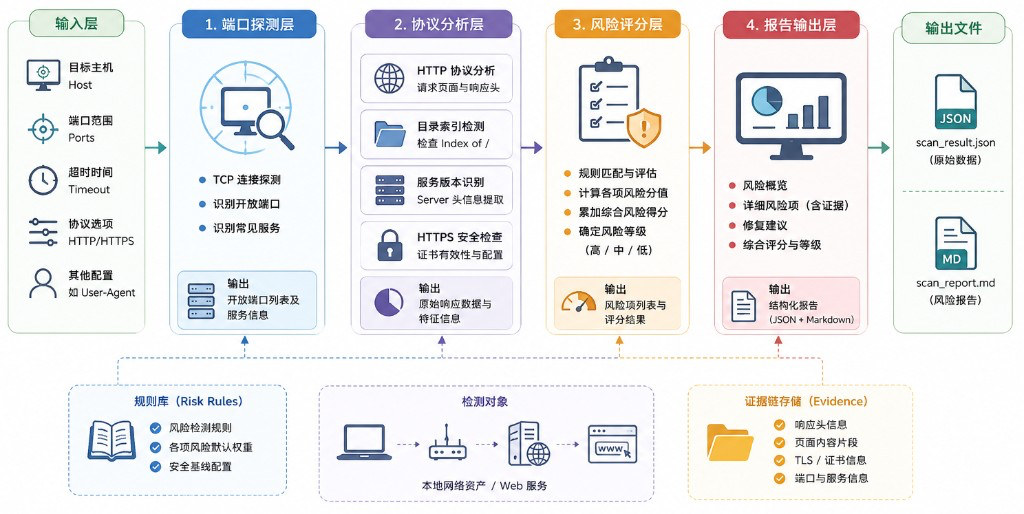
\includegraphics[width=0.95\textwidth]{figures/architecture.png}
  \caption{系统总体架构图}
  \label{fig:architecture}
\end{figure}

图 \ref{fig:architecture} 展示了系统的总体架构，按照“输入层、端口探测层、协议分析层、风险评分层、报告输出层”的顺序组织，并辅以规则库、检测对象与证据链存储等支撑组件。该结构便于阅读者快速理解系统模块边界与各模块之间的数据流关系。

\subsection{系统架构}

系统总体上划分为四层：

\begin{enumerate}[label=\arabic*.]
  \item 端口探测层：通过 Socket 判断目标端口是否开放；
  \item 协议分析层：对开放服务发起 HTTP/HTTPS 请求，提取响应头、页面摘要、证书和 TLS 参数；
  \item 风险评分层：依据规则库生成风险项并计算综合分值；
  \item 报告输出层：生成结构化 JSON 和可读性较强的 Markdown 文档。
\end{enumerate}

该架构的优点在于职责清晰。端口探测层解决“是否存在服务”，协议分析层回答“服务返回了什么”，风险评分层解释“这些返回意味着什么”，报告输出层则将结果转化为适合阅读和归档的内容。

进一步来看，该架构实际上兼顾了“检测流程线性化”和“规则逻辑模块化”两种需求。一方面，扫描过程沿着网络访问链路逐步推进，天然适合按阶段组织；另一方面，不同风险规则又可以独立追加到分析层与评分层中，从而避免系统因功能扩展而出现整体耦合过高的问题。这种设计虽然属于轻量级实现，但已经能够支撑本文所需的风险识别、证据生成和结果输出。

\subsection{模块划分}

结合具体实现，系统包含以下核心模块：

\begin{enumerate}[label=\arabic*.]
  \item 参数解析模块：处理目标主机、端口集合、超时参数与输出路径；
  \item 端口扫描模块：基于 TCP 连接状态识别开放端口；
  \item HTTP 风险检测模块：关注目录索引、版本暴露和安全头缺失问题；
  \item HTTPS 风险检测模块：关注握手异常、证书时效和 TLS 协议安全性；
  \item 风险汇总模块：负责分值统计、等级判定与报告生成。
\end{enumerate}

\subsection{数据结构设计}

系统中定义了两个核心数据对象，即 \texttt{PortResult} 与 \texttt{Finding}。其中，\texttt{PortResult} 用于描述端口号、开放状态、服务类型和风险提示；\texttt{Finding} 用于描述具体风险项，包括标题、严重级别、风险分值、证据与整改建议。

这种设计方式将“扫描结果”与“风险结论”解耦，使得程序既可以在底层保留原始探测信息，又可以在上层灵活扩展分析规则。例如，未来若增加弱口令探测、目录枚举或组件指纹识别等功能，只需新增对应的风险生成逻辑，而无需重构现有数据模型。

\subsection{风险评分模型}

本文采用规则驱动的风险评分模型，将不同问题映射为不同分值。设单项风险分值为 $s_i$，则综合风险分值可定义为：

\begin{equation}
S = \sum_{i=1}^{n} s_i
\end{equation}

在此基础上，系统进一步结合高风险项数量对整体等级进行划分：当总分较高或高风险项数量较多时，判定为高风险；当存在一定数量的中高风险项时，判定为中风险；其余情况判定为低风险。

该模型虽然简化了现实场景中资产价值、暴露范围和业务重要性等因素，但它能够在本地实验条件下实现直观、可解释的量化输出，满足本文对风险比较和等级判定的需求。

\begin{algorithm}[H]
\caption{风险评分与等级判定算法}
\label{alg:risk-score}
\begin{algorithmic}[1]
\Require 风险项集合 $F=\{f_1,f_2,\dots,f_n\}$
\Ensure 综合风险分值 $S$ 与总体风险等级 $L$
\State $S \gets 0$
\State $H \gets 0$, $M \gets 0$, $L_c \gets 0$
\For{每个风险项 $f_i \in F$}
  \State $S \gets S + score(f_i)$
  \If{$severity(f_i)=high$}
    \State $H \gets H + 1$
  \ElsIf{$severity(f_i)=medium$}
    \State $M \gets M + 1$
  \Else
    \State $L_c \gets L_c + 1$
  \EndIf
\EndFor
\If{$S \geq 80$ \textbf{or} $H \geq 3$}
  \State $L \gets$ 高风险
\ElsIf{$S \geq 40$ \textbf{or} $H \geq 1$ \textbf{or} $M \geq 4$}
  \State $L \gets$ 中风险
\Else
  \State $L \gets$ 低风险
\EndIf
\State \Return $(S, L)$
\end{algorithmic}
\end{algorithm}

算法 \ref{alg:risk-score} 描述了本文采用的风险评分与等级判定过程。该算法的核心思想是先对全部风险项进行累积分值统计，再结合高风险项和中风险项数量做分层判断。与单纯依赖总分的判定方式相比，这种“分值 + 风险等级分布”的组合策略更符合安全分析的直觉：即便总分尚未极端偏高，只要出现若干高风险问题，整体安全状态也不应被低估。

\subsection{设计原则与关键权衡}

在系统设计过程中，本文对若干设计选择进行了权衡，最终确定了适合本文目标的轻量化方案，具体说明如下。

\textbf{（1）标准库优先原则}

系统全程只使用 Python 标准库（\texttt{socket}、\texttt{ssl}、\texttt{http.client} 等），未引入任何第三方包。这一选择带来了两方面好处：其一，在任何安装了 Python 3 的环境中均可直接运行，无需 \texttt{pip install}，降低了部署门槛；其二，代码中没有被第三方库封装的"黑盒"调用，每一步网络交互都可以追溯到具体的标准库函数，充分体现了自主编程的要求。代价是部分高级功能（如异步扫描、TLS 指纹识别）需要自行实现，当前版本未完全覆盖。

\textbf{（2）同步串行 vs 异步并发}

端口扫描采用了同步串行方式，即逐个端口依次发起连接探测，而非多线程或异步并发扫描。对于本文设定的本地检测范围，端口数量通常在个位数到十几个之间，串行方式的总耗时通常不超过几秒，能够满足验证需求，且代码逻辑清晰、易于调试。若未来需要扫描数百个端口，只需将主循环替换为 \texttt{concurrent.futures.ThreadPoolExecutor}，无需对函数逻辑做任何修改，因此串行设计不构成扩展障碍。

\textbf{（3）规则驱动 vs 机器学习}

风险识别逻辑完全由人工定义的规则驱动，而未采用机器学习方法。对于"响应头是否存在"、"TLS版本是否过旧"这类问题，本质上是确定性的布尔判断，不存在需要模型拟合的概率分布，规则驱动方式反而更简洁、更可解释。此外，规则库可以通过修改字典随时扩展，无需重新训练模型，更适合轻量级原型系统的迭代需求。

\textbf{（4）双格式报告输出}

系统同时输出 JSON 和 Markdown 两种格式，而非只选其一。JSON 格式结构清晰、机器可读，适合后续脚本处理或接入可视化平台；Markdown 格式人类可读，可以通过 \texttt{pandoc} 或 \texttt{xelatex} 直接转换为 PDF 提交。两种格式在代码层面共享同一份检测结果数据，额外开销极小，而带来的使用灵活性则较为显著。

\section{系统实现}

\subsection{实现环境}

系统以 Python 3 为开发语言，尽量使用标准库完成全部核心逻辑。主要使用到的库包括：

\begin{itemize}
  \item \texttt{socket}：用于端口连通性探测；
  \item \texttt{ssl}：用于 TLS 握手、证书信息与密码套件提取；
  \item \texttt{http.client}：用于构造 HTTP/HTTPS 请求；
  \item \texttt{argparse}：用于命令行参数解析；
  \item \texttt{json}：用于结构化结果导出；
  \item \texttt{dataclasses}：用于封装结果对象。
\end{itemize}

这种实现策略能够突出自主编程实现的特点，避免系统实质上退化为对第三方工具的调用封装。

\subsection{规则库与核心数据结构定义}

在系统实现之前，需要先定义两类静态规则库与两个核心数据类，它们是整个检测逻辑的基础。

\textbf{端口风险规则库 \texttt{RISK\_PORTS}}：该字典将常见敏感端口映射为服务名称、风险提示和基础分值三元组。基础分值越高，表示该端口一旦开放所带来的暴露面风险越严重。例如 Redis（6379）直接暴露可能导致未授权访问和数据库清空，赋予最高基础分值 30；Telnet（23）明文传输远程管理凭据，赋予 25 分；FTP（21）和 MySQL（3306）各赋 20 分。443（HTTPS）与 8443（HTTPS-Alt）的基础分值均为 0，因为 HTTPS 端口本身并非暴露面风险，其安全性需要由 4.6 节的协议层检测模块进一步判定。

\begin{lstlisting}[language=Python,caption={端口风险规则库定义}]
RISK_PORTS: Dict[int, tuple[str, str, int]] = {
    21:   ("FTP",       "FTP 明文传输账号口令，存在被嗅探风险。",            20),
    23:   ("Telnet",    "Telnet 明文传输，远程管理风险较高。",               25),
    80:   ("HTTP",      "仅暴露 HTTP 可能导致流量明文传输。",               10),
    443:  ("HTTPS",     "HTTPS 端口正常，但仍需检查证书与安全头。",            0),
    3306: ("MySQL",     "数据库端口直接暴露可能带来弱口令和越权访问风险。",    20),
    6379: ("Redis",     "Redis 端口若未鉴权直接暴露，风险极高。",            30),
    8080: ("HTTP-Alt",  "备用 Web 端口常用于测试服务，配置疏漏概率较高。",    10),
    8443: ("HTTPS-Alt", "备用 HTTPS 端口常用于测试环境，需重点核查证书可信性与协议配置。", 0),
}
\end{lstlisting}

\textbf{安全响应头规则库 \texttt{SECURITY\_HEADERS}}：该字典定义了需要检测的 HTTP 安全响应头名称与对应的风险分值。分值设计依据各响应头的防护价值：HSTS 和 CSP 对 HTTPS 强制与 XSS 防护作用最大，各赋 10 分；X-Frame-Options 防点击劫持赋 8 分；X-Content-Type-Options 防 MIME 嗅探赋 6 分；Referrer-Policy 防来源泄露赋 4 分。

\begin{lstlisting}[language=Python,caption={安全响应头规则库定义}]
SECURITY_HEADERS = {
    "Strict-Transport-Security": 10,
    "Content-Security-Policy":   10,
    "X-Frame-Options":            8,
    "X-Content-Type-Options":     6,
    "Referrer-Policy":            4,
}
\end{lstlisting}

\textbf{数据类 \texttt{PortResult} 与 \texttt{Finding}}：系统使用 Python 的 \texttt{dataclass} 装饰器定义两个核心数据对象，以结构化方式封装检测结果。

\begin{lstlisting}[language=Python,caption={核心数据结构定义}]
@dataclass
class Finding:
    title:          str   # 风险标题
    severity:       str   # 严重级别: high / medium / low
    score:          int   # 风险分值
    evidence:       str   # 证据描述
    recommendation: str   # 整改建议

@dataclass
class PortResult:
    port:      int   # 端口号
    open:      bool  # 是否开放
    service:   str   # 服务类型
    risk_hint: str   # 风险提示
\end{lstlisting}

使用 \texttt{dataclass} 的好处在于：其一，字段定义清晰，可直接通过 \texttt{asdict()} 序列化为字典，方便后续 JSON 导出；其二，与普通字典相比，数据类提供了类型注解和字段级别的访问约束，有利于后续功能扩展时保持接口一致性。

\subsection{端口扫描实现}

端口扫描模块通过创建 TCP Socket 并调用 \texttt{connect\_ex()} 检测目标端口是否开放。若返回值为 0，则表示目标端口在当前网络上下文中可访问。该逻辑如代码片段所示。

\begin{lstlisting}[language=Python,caption={端口扫描核心逻辑}]
def scan_port(host: str, port: int, timeout: float) -> PortResult:
    service, risk_hint, _ = RISK_PORTS.get(
        port, ("Unknown", "未知服务，请结合实际业务研判。", 5)
    )
    sock = socket.socket(socket.AF_INET, socket.SOCK_STREAM)
    sock.settimeout(timeout)
    try:
        open_flag = sock.connect_ex((host, port)) == 0
    finally:
        sock.close()
    return PortResult(port=port, open=open_flag, service=service, risk_hint=risk_hint)
\end{lstlisting}

在此基础上，程序还结合预设端口字典对敏感服务进行简单映射，例如对 21、23、3306、6379 和 8080 等端口给出不同风险提示，以提升检测结果的解释能力。

\begin{algorithm}[H]
\caption{端口扫描算法}
\label{alg:port-scan}
\begin{algorithmic}[1]
\Require 目标主机 $host$，端口集合 $P=\{p_1,p_2,\dots,p_m\}$，超时时间 $t$
\Ensure 端口结果集合 $R$
\State 初始化结果集合 $R \gets \emptyset$
\For{每个端口 $p_i \in P$}
  \State 创建 TCP Socket 并设置超时时间为 $t$
  \State 尝试连接 $(host, p_i)$
  \If{连接成功}
    \State 记录该端口状态为 open
  \Else
    \State 记录该端口状态为 closed
  \EndIf
  \State 根据预设端口映射表生成服务类型与基础风险提示
  \State 将结果加入集合 $R$
\EndFor
\State \Return $R$
\end{algorithmic}
\end{algorithm}

从算法层面看，端口扫描模块虽然采用串行实现，但其逻辑链路十分清晰，适合作为整个检测系统的入口。更重要的是，端口扫描结果并非最终输出，而是作为后续协议分析的筛选条件。只有当目标端口处于开放状态时，系统才继续进入 HTTP 或 HTTPS 检查阶段，因此该模块在整体流程中承担着“缩小分析范围、降低无效请求数量”的作用。

\subsection{HTTP 请求辅助模块实现}

在执行 HTTP 或 HTTPS 风险检测之前，系统需要先向目标服务发起一次 GET 请求，获取响应头和页面正文预览。该功能由 \texttt{request\_headers()} 函数统一封装，供后续 HTTP 与 HTTPS 检测模块复用。

\begin{lstlisting}[language=Python,caption={HTTP/HTTPS 请求辅助函数}]
def request_headers(
    host: str, port: int, use_https: bool, timeout: float
) -> Optional[dict]:
    conn_cls = HTTPSConnection if use_https else HTTPConnection
    if use_https:
        context = ssl.create_default_context()
        conn = conn_cls(host, port=port, timeout=timeout, context=context)
    else:
        conn = conn_cls(host, port=port, timeout=timeout)
    try:
        conn.request("GET", "/")
        resp = conn.getresponse()
        headers = {k: v for k, v in resp.getheaders()}
        body = resp.read(512).decode("utf-8", errors="ignore")
        headers["_status"] = str(resp.status)
        headers["_preview"] = body   # 保存正文前 512 字节供规则匹配
        return headers
    except Exception:
        return None     # 连接失败返回 None，上层模块直接跳过
    finally:
        conn.close()
\end{lstlisting}

该函数的设计有几个关键点：

\begin{enumerate}[label=\arabic*.]
  \item \textbf{HTTP/HTTPS 统一接口}：通过 \texttt{use\_https} 参数控制连接类型，上层模块无需关心协议差异，只需传入不同标志即可复用同一套请求逻辑；
  \item \textbf{正文截断预览}：正文读取上限为 512 字节（\texttt{resp.read(512)}），足以匹配目录索引暴露的 \texttt{Index of /} 特征，同时避免下载超大页面导致的性能问题；
  \item \textbf{异常静默处理}：若目标端口连接超时或拒绝连接，函数返回 \texttt{None} 而非抛出异常，调用方通过判断返回值是否为 \texttt{None} 决定是否跳过后续分析，保证扫描流程的健壮性；
  \item \textbf{内置字段扩展}：将 HTTP 状态码（\texttt{\_status}）和正文预览（\texttt{\_preview}）以约定前缀存入同一字典，避免额外定义数据类，简化了跨模块的数据传递。
\end{enumerate}

\subsection{HTTP 风险检测实现}

HTTP 风险检测模块首先使用 \texttt{HTTPConnection} 发起请求并获取响应头与页面预览，再根据规则判断是否存在安全头缺失、目录索引暴露和版本信息泄露等问题。其核心思路包括：

\begin{enumerate}[label=\arabic*.]
  \item 读取 \texttt{Server} 头，判断是否包含精确版本信息；
  \item 遍历预设安全响应头集合，识别缺失项；
  \item 对响应正文进行快速预览，匹配 \texttt{Index of /} 等目录暴露特征。
\end{enumerate}

\begin{lstlisting}[language=Python,caption={HTTP 风险检测逻辑}]
def check_http_service(host: str, port: int, timeout: float) -> List[Finding]:
    findings: List[Finding] = []
    headers = request_headers(host, port, use_https=False, timeout=timeout)
    if not headers:
        return findings

    server = headers.get("Server", "未返回")
    if server and "/" in server:
        findings.append(
            Finding(
                title="Server 版本信息暴露",
                severity="medium",
                score=8,
                evidence=f"端口 {port} 返回 Server 头: {server}",
                recommendation="隐藏精确版本号，仅保留必要产品标识。"
            )
        )

    for header, score in SECURITY_HEADERS.items():
        if header not in headers:
            findings.append(
                Finding(
                    title=f"缺少安全响应头 {header}",
                    severity="medium" if score >= 8 else "low",
                    score=score,
                    evidence=f"端口 {port} 响应中未发现 {header}",
                    recommendation=f"在 Web 服务或反向代理中补充 {header} 配置。"
                )
            )

    preview = headers.get("_preview", "").lower()
    if "index of /" in preview:
        findings.append(
            Finding(
                title="疑似目录索引暴露",
                severity="high",
                score=20,
                evidence=f"端口 {port} 页面内容包含 'Index of /'",
                recommendation="关闭目录浏览功能，避免静态资源、日志或备份文件被遍历获取。"
            )
        )

    return findings
\end{lstlisting}

可以看到，该函数完整覆盖了算法 \ref{alg:http-check} 描述的三个判定环节：版本信息暴露判定、安全响应头逐项遍历、目录索引特征匹配，三者共用同一份 \texttt{headers} 数据，避免了重复请求。这一实现使系统从单纯的“端口开放检测”扩展到了“服务配置风险检测”，更符合网络安全巡检的实际需求。

\begin{algorithm}[H]
\caption{HTTP 风险检测算法}
\label{alg:http-check}
\begin{algorithmic}[1]
\Require 目标主机 $host$，端口 $port$
\Ensure HTTP 风险项集合 $F_h$
\State 发起 HTTP GET 请求并获取响应头与页面预览内容
\If{请求失败}
  \State 返回空集合
\EndIf
\If{Server 头包含精确版本信息}
  \State 生成版本信息暴露风险项
\EndIf
\For{每个预定义安全响应头}
  \If{该响应头不存在}
    \State 生成对应的安全头缺失风险项
  \EndIf
\EndFor
\If{页面正文包含 ``Index of /'' 特征}
  \State 生成目录索引暴露风险项
\EndIf
\State \Return $F_h$
\end{algorithmic}
\end{algorithm}

算法 \ref{alg:http-check} 的价值在于，它把常见 Web 基础安全问题编码为一组明确可执行的判定规则。对于本文而言，这种规则集合的设计意义并不只是“能扫出问题”，更在于它把日常经验性的安全检查动作转换成了可复现、可复用、可维护的程序逻辑。换言之，本文不仅实现了一个工具，更实现了一套基础风险知识的程序化表达方式。

\subsection{HTTPS 风险检测实现}

对于 HTTPS 服务，系统首先利用 \texttt{ssl.create\_default\_context()} 建立采用严格证书校验的 TLS 连接。该上下文会同时校验证书链的可信性与服务端主机名，是绝大多数 HTTPS 客户端的默认行为。然而，在真实网络环境中，最常见的 HTTPS 配置问题并不是“完全无法握手”，而是“握手过程中证书校验失败”——例如使用自签名证书、证书已过期或证书链不完整等。早期版本的实现将这些情况一律归入“握手失败或证书异常”这一笼统类别，既无法区分具体原因，也无法继续提取协议版本与密码套件等有价值信息。

为此，本系统采用\textbf{两阶段握手策略}：第一阶段使用严格校验上下文尝试连接，若因证书校验失败抛出 \texttt{ssl.SSLCertVerificationError}，系统会读取该异常自带的 \texttt{verify\_code} 与 \texttt{verify\_message} 属性——这两个字段直接来自 OpenSSL 的证书链校验结果，例如 \texttt{verify\_code=18} 对应“self-signed certificate”——并据此生成更具体的风险项（自签名证书、证书已过期或证书链校验失败）。随后，系统进入第二阶段，使用 \texttt{verify\_mode=ssl.CERT\_NONE} 的非校验上下文重新握手，在不依赖证书可信性的前提下继续提取 TLS 协议版本与密码套件，使后续的协议版本检查与弱密码套件检查依然能够执行。这一策略完全基于标准库 \texttt{ssl} 模块的公开接口实现，未引入任何第三方依赖。

\begin{lstlisting}[language=Python,caption={证书校验失败原因分类}]
SELF_SIGNED_VERIFY_CODES = {18, 19}

def _classify_cert_verification_error(
    host: str, port: int, exc: ssl.SSLCertVerificationError
) -> Finding:
    code = exc.verify_code
    message = exc.verify_message or str(exc)
    if code in SELF_SIGNED_VERIFY_CODES or "self signed" in message or "self-signed" in message:
        return Finding(
            title="HTTPS 证书为自签名证书",
            severity="medium",
            score=12,
            evidence=f"{host}:{port} 证书校验失败：{message}（verify_code={code}）",
            recommendation="改用受信任 CA 签发的证书；如为内网场景，应部署私有 CA 并将根证书分发至客户端信任库。"
        )
    if "expired" in message:
        return Finding(
            title="HTTPS 证书已过期",
            severity="high",
            score=25,
            evidence=f"{host}:{port} 证书校验失败：{message}（verify_code={code}）",
            recommendation="立即更新证书并检查自动续期机制。"
        )
    return Finding(
        title="HTTPS 证书链校验失败",
        severity="medium",
        score=15,
        evidence=f"{host}:{port} 证书校验失败：{message}（verify_code={code}）",
        recommendation="检查证书链完整性，确认中间证书已正确部署，并核实证书与访问域名是否匹配。"
    )
\end{lstlisting}

\begin{lstlisting}[language=Python,caption={HTTPS 风险检测逻辑}]
def check_https_service(host: str, port: int, timeout: float) -> List[Finding]:
    findings: List[Finding] = []
    cert: dict = {}
    cipher = None
    version = None

    context = ssl.create_default_context()
    try:
        with socket.create_connection((host, port), timeout=timeout) as sock:
            with context.wrap_socket(sock, server_hostname=host) as wrapped:
                cert = wrapped.getpeercert()
                cipher = wrapped.cipher()
                version = wrapped.version()
    except ssl.SSLCertVerificationError as exc:
        # 证书校验失败：先记录具体原因，再用非校验上下文重新握手
        findings.append(_classify_cert_verification_error(host, port, exc))
        try:
            insecure_context = ssl.SSLContext(ssl.PROTOCOL_TLS_CLIENT)
            insecure_context.check_hostname = False
            insecure_context.verify_mode = ssl.CERT_NONE
            with socket.create_connection((host, port), timeout=timeout) as sock:
                with insecure_context.wrap_socket(sock, server_hostname=host) as wrapped:
                    cert = wrapped.getpeercert()
                    cipher = wrapped.cipher()
                    version = wrapped.version()
        except Exception:
            return findings
    except Exception as exc:
        findings.append(
            Finding(
                title="HTTPS 握手失败或证书异常",
                severity="high",
                score=25,
                evidence=f"连接 {host}:{port} 时出现异常: {exc}",
                recommendation="检查 TLS 配置、证书链和服务监听状态。"
            )
        )
        return findings

    if version in {"TLSv1", "TLSv1.1"}:
        findings.append(
            Finding(
                title="TLS 协议版本过旧",
                severity="high",
                score=20,
                evidence=f"服务端协商出的 TLS 版本为 {version}",
                recommendation="停用 TLS 1.0/1.1，仅保留 TLS 1.2 及以上版本。"
            )
        )

    if cipher:
        cipher_name = cipher[0]
        if "RC4" in cipher_name or "3DES" in cipher_name:
            findings.append(
                Finding(
                    title="加密套件强度不足",
                    severity="high",
                    score=18,
                    evidence=f"当前协商密码套件为 {cipher_name}",
                    recommendation="关闭弱加密套件，启用现代 AEAD 套件。"
                )
            )

    not_after = cert.get("notAfter")
    if not_after:
        expire_at = parsedate_to_datetime(not_after)
        now = datetime.now(timezone.utc)
        days_left = (expire_at - now).days
        if days_left < 0:
            findings.append(
                Finding(
                    title="HTTPS 证书已过期",
                    severity="high",
                    score=25,
                    evidence=f"证书过期时间为 {expire_at.isoformat()}",
                    recommendation="立即更新证书并检查自动续期机制。"
                )
            )
        elif days_left <= 30:
            findings.append(
                Finding(
                    title="HTTPS 证书即将到期",
                    severity="medium",
                    score=10,
                    evidence=f"证书剩余有效期 {days_left} 天",
                    recommendation="提前续签证书，避免服务中断。"
                )
            )

    return findings
\end{lstlisting}

上述两个函数共同实现了算法 \ref{alg:https-check} 中的五类判定：证书校验失败原因分类（自签名 / 已过期 / 证书链异常）、握手异常兜底、TLS 协议版本检查、密码套件强度检查与证书有效期检查。其中证书有效期判断借助标准库 \texttt{email.utils.parsedate\_to\_datetime} 将证书 \texttt{notAfter} 字段解析为带时区的 \texttt{datetime} 对象，再与当前 UTC 时间相减得到剩余天数 \texttt{days\_left}，分别对应“已过期”（高风险）和“即将到期”（中风险，剩余不超过 30 天）两种情形。需要说明的是，在 \texttt{verify\_mode=ssl.CERT\_NONE} 的非校验握手下，\texttt{getpeercert()} 默认返回空字典，因此证书有效期检查仅在证书可被正常解析（即第一阶段握手直接成功）时才会执行，这是该实现在标准库范围内的一个已知边界，将在 5.7 节实验中具体讨论。

\begin{algorithm}[H]
\caption{HTTPS 风险检测算法}
\label{alg:https-check}
\begin{algorithmic}[1]
\Require 目标主机 $host$，端口 $port$
\Ensure HTTPS 风险项集合 $F_s$
\State 使用严格证书校验上下文尝试建立 TLS 连接并完成握手
\If{握手因证书校验失败抛出异常}
  \State 读取异常的 verify\_code 与 verify\_message
  \If{校验码对应自签名证书}
    \State 生成“证书为自签名证书”风险项
  \ElsIf{校验信息提示证书已过期}
    \State 生成“证书已过期”风险项
  \Else
    \State 生成“证书链校验失败”风险项
  \EndIf
  \State 使用不校验证书的上下文重新握手以获取协议版本与密码套件
  \If{重新握手仍失败}
    \State \Return $F_s$
  \EndIf
\ElsIf{握手因其他原因失败}
  \State 生成 HTTPS 握手失败或证书异常风险项
  \State \Return $F_s$
\EndIf
\State 提取（或重新获取）证书信息、TLS 版本与密码套件
\If{证书已过期}
  \State 生成证书过期风险项
\ElsIf{证书剩余有效期小于阈值}
  \State 生成证书即将过期风险项
\EndIf
\If{TLS 版本为 TLS 1.0 或 TLS 1.1}
  \State 生成老旧协议风险项
\EndIf
\If{密码套件包含 RC4 或 3DES}
  \State 生成弱密码套件风险项
\EndIf
\State \Return $F_s$
\end{algorithmic}
\end{algorithm}

相较于早期版本，该算法的改进之处在于：将“证书不可信”从“连接异常”中分离出来，单独作为一类可解释、可量化的风险项。这一调整具有现实意义——根据安全社区的普遍经验，自签名证书是内网与测试环境中最常见的 HTTPS 配置问题之一，其本质并非“服务不可达”，而是“服务可达但身份无法验证”，理应被作为独立风险呈现给使用者，而不是与网络连通性故障混为一谈。第 5.7 节的实验四将基于本地自签名证书演示服务，对该算法的执行结果进行完整验证。

\subsection{端口风险计算模块实现}

端口扫描完成后，需要将开放端口映射为具体的 \texttt{Finding} 风险项。该模块遍历所有端口扫描结果，对处于开放状态且在 \texttt{RISK\_PORTS} 字典中存在记录的端口生成对应风险项。

\begin{lstlisting}[language=Python,caption={端口风险计算模块}]
def calculate_port_risk(results: List[PortResult]) -> List[Finding]:
    findings: List[Finding] = []
    for result in results:
        if not result.open:
            continue  # 端口未开放，直接跳过
        _, hint, base_score = RISK_PORTS.get(
            result.port, ("Unknown", result.risk_hint, 5)
        )
        if base_score > 0:
            severity = "high" if base_score >= 20 else "medium"
            findings.append(
                Finding(
                    title=f"开放端口 {result.port} 暴露风险",
                    severity=severity,
                    score=base_score,
                    evidence=f"{result.port}/{result.service} 处于开放状态。{hint}",
                    recommendation=(
                        "确认端口是否必须对外开放；"
                        "若非必要，应关闭或限制访问来源。"
                    ),
                )
            )
    return findings
\end{lstlisting}

该模块的设计体现了规则驱动的思想：风险的判定依据完全来自 \texttt{RISK\_PORTS} 字典，添加新的高风险端口只需在字典中追加一条记录，无需修改函数逻辑本身。严重级别的划分也遵循统一标准：基础分值 $\geq 20$ 的端口（如 FTP、Telnet、MySQL、Redis）标记为高风险，其余标记为中风险。

\subsection{风险汇总与等级判定模块实现}

所有 \texttt{Finding} 对象收集完毕后，由 \texttt{summarize()} 函数进行统计汇总，计算综合评分并判定整体风险等级。

\begin{lstlisting}[language=Python,caption={风险汇总与等级判定模块}]
def summarize(findings: List[Finding]) -> dict:
    total  = sum(item.score for item in findings)
    high   = sum(1 for item in findings if item.severity == "high")
    medium = sum(1 for item in findings if item.severity == "medium")
    low    = sum(1 for item in findings if item.severity == "low")

    if total >= 80 or high >= 3:
        level = "高风险"
    elif total >= 40 or high >= 1 or medium >= 4:
        level = "中风险"
    else:
        level = "低风险"

    return {
        "total_score":   total,
        "risk_level":    level,
        "high_count":    high,
        "medium_count":  medium,
        "low_count":     low,
    }
\end{lstlisting}

该函数实现了算法 \ref{alg:risk-score} 中描述的评分逻辑。等级判定采用“分值优先、高危数量兜底”的组合策略：
\begin{itemize}
  \item 若总分 $\geq 80$ 或高风险项 $\geq 3$ 个，判定为高风险；
  \item 若总分 $\geq 40$，或存在至少 1 个高风险项，或中风险项 $\geq 4$ 个，判定为中风险；
  \item 其余情况判定为低风险。
\end{itemize}

这一设计的合理性在于：即使总分尚未达到 80，只要存在若干高风险问题（如直接暴露的 Redis 或过期证书），整体安全状态同样不应被低估，因此高危数量兜底条件的引入符合安全分析的实际直觉。

\subsection{报告生成模块实现}

为保证执行结果和风险展示均可复核，系统在运行结束后自动输出两类文件。一类是 \texttt{scan\_result.json}，用于保存完整结构化数据；另一类是 \texttt{scan\_report.md}，用于生成面向阅读的文本报告。这样既便于机器处理，也便于人工分析和后续文档整理。

从结果工程化的角度看，结构化输出与文档化输出并行是非常重要的设计选择。前者便于脚本继续处理，例如批量汇总多台主机结果、后续接入数据库或进行图表统计；后者则更适合论文分析、归档复核以及安全分析人员快速阅读。通过同时保留这两种输出形式，系统不仅能够证明程序已完成运行，也兼顾了结果可使用、可展示、可追溯的实践需求。

Markdown 报告由 \texttt{generate\_markdown()} 函数生成，其核心逻辑如下：

\begin{lstlisting}[language=Python,caption={Markdown 报告生成函数}]
def generate_markdown(
    host: str,
    ports: List[PortResult],
    findings: List[Finding],
    summary: dict
) -> str:
    lines = [
        "# 本地网络资产与 Web 安全配置风险检测报告",
        f"- 扫描目标：`{host}`",
        f"- 风险等级：`{summary['risk_level']}`",
        f"- 综合分值：`{summary['total_score']}`",
        "",
        "## 端口扫描结果",
        "| 端口 | 状态 | 服务 | 风险提示 |",
        "| --- | --- | --- | --- |",
    ]
    for item in ports:
        state = "open" if item.open else "closed"
        lines.append(f"| {item.port} | {state} | {item.service} | {item.risk_hint} |")

    lines.extend(["", "## 风险明细", ""])
    if not findings:
        lines.append("未发现显著风险。")
    else:
        for idx, item in enumerate(findings, 1):
            lines.extend([
                f"### {idx}. {item.title}",
                f"- 严重级别：`{item.severity}`",
                f"- 风险分值：`{item.score}`",
                f"- 证据：{item.evidence}",
                f"- 建议：{item.recommendation}",
                "",
            ])

    lines.extend([
        "## 统计摘要",
        f"- 高风险：{summary['high_count']} 项",
        f"- 中风险：{summary['medium_count']} 项",
        f"- 低风险：{summary['low_count']} 项",
    ])
    return "\n".join(lines)
\end{lstlisting}

该函数的设计采用字符串列表拼接方式，逐节构建 Markdown 文档，最终通过 \texttt{"\textbackslash n".join(lines)} 合并输出，避免了大量字符串拼接带来的性能问题。报告分为三个区块：扫描摘要信息、端口扫描结果表格和按序号排列的风险明细，每条风险项均包含标题、级别、分值、证据和整改建议，结构清晰、便于阅读。

\subsection{演示环境实现}

为了验证检测逻辑的有效性，本文编写了一个弱安全配置演示服务。该服务监听本地 8080 端口，主动返回包含版本信息的 \texttt{Server} 头，不设置常见安全响应头，并构造带有 \texttt{Index of /} 特征的页面内容。核心片段如下：

\begin{lstlisting}[language=Python,caption={本地弱配置演示服务}]
class VulnerableHandler(BaseHTTPRequestHandler):
    server_version = "Apache/2.4.49"

    def do_GET(self) -> None:
        body = """
        <html>
          <head><title>Index of /</title></head>
          <body>
            <h1>Index of /</h1>
            <ul>
              <li><a href="/backup.zip">backup.zip</a></li>
              <li><a href="/logs/">logs/</a></li>
              <li><a href="/config/">config/</a></li>
            </ul>
          </body>
        </html>
        """.encode("utf-8")
\end{lstlisting}

通过该演示环境，系统可以在本地稳定复现实验过程并输出具有代表性的检测结果。

为配合 4.6 节描述的 HTTPS 检测模块，本文进一步在同一演示程序中增加了一个基于自签名证书的 HTTPS 监听端口（8443）。证书与私钥通过 \texttt{openssl} 命令行工具一次性生成，并保存为 \texttt{demo\_certs/cert.pem} 与 \texttt{demo\_certs/key.pem}：

\begin{lstlisting}[language=bash]
openssl req -x509 -newkey rsa:2048 -nodes -days 825 \
  -keyout demo_certs/key.pem -out demo_certs/cert.pem \
  -subj "/C=CN/ST=Beijing/L=Beijing/O=NormalTime Lab/CN=127.0.0.1" \
  -addext "subjectAltName=IP:127.0.0.1"
\end{lstlisting}

证书生成是一次性的环境准备步骤，由系统管理员在部署演示环境时手动执行，与 \texttt{risk\_scanner.py} 的检测逻辑本身无关，因此不影响该程序“仅依赖标准库”的实现原则。演示程序在启动时加载该证书，使用标准库 \texttt{ssl.SSLContext} 将普通 \texttt{ThreadingHTTPServer} 的监听套接字包装为 TLS 套接字：

\begin{lstlisting}[language=Python,caption={基于自签名证书的 HTTPS 演示服务}]
def start_https_server() -> ThreadingHTTPServer | None:
    cert_file = CERT_DIR / "cert.pem"
    key_file = CERT_DIR / "key.pem"
    if not (cert_file.exists() and key_file.exists()):
        print(f"未找到自签名证书 {cert_file}，跳过 HTTPS 演示服务。")
        return None

    handler = partial(VulnerableHandler, directory=str(DEMO_ROOT))
    server = ThreadingHTTPServer(("127.0.0.1", 8443), handler)
    context = ssl.SSLContext(ssl.PROTOCOL_TLS_SERVER)
    context.load_cert_chain(certfile=str(cert_file), keyfile=str(key_file))
    server.socket = context.wrap_socket(server.socket, server_side=True)
    print("Demo vulnerable server (self-signed HTTPS) running on https://127.0.0.1:8443")
    return server
\end{lstlisting}

由于该证书为自签名证书（证书的颁发者与使用者相同），任何使用默认信任库的 HTTPS 客户端在与 8443 端口握手时都会触发证书校验失败，这正是 4.6 节两阶段握手策略所要处理的典型场景。该 HTTPS 演示监听器与 8080 端口的 HTTP 演示服务在同一进程中以独立线程运行，二者共用同一份演示页面内容，便于在一次实验中同时观察 HTTP 与 HTTPS 两类检测结果。

\subsection{主程序控制流实现}

\texttt{main()} 函数是整个系统的入口，负责将参数解析、端口扫描、风险检测、汇总评分与报告输出各模块串联为完整的执行流水线。

\begin{lstlisting}[language=Python,caption={主程序控制流}]
def main() -> int:
    args = parse_args()
    ports = [int(p.strip()) for p in args.ports.split(",") if p.strip()]

    # 阶段一：端口扫描
    scan_results = [scan_port(args.host, p, args.timeout) for p in ports]

    # 阶段二：协议层风险检测
    findings = calculate_port_risk(scan_results)
    for item in scan_results:
        if item.open and item.port in {80, 8000, 8080}:
            findings.extend(check_http_service(args.host, item.port, args.timeout))
        if item.open and item.port in {443, 8443}:
            findings.extend(check_https_service(args.host, item.port, args.timeout))

    # 阶段三：排序、汇总与等级判定
    findings.sort(key=lambda x: x.score, reverse=True)
    summary = summarize(findings)

    # 阶段四：报告输出
    output_dir = Path(args.output_dir)
    output_dir.mkdir(parents=True, exist_ok=True)
    payload = {
        "target": args.host,
        "ports": [asdict(item) for item in scan_results],
        "findings": [asdict(item) for item in findings],
        "summary": summary,
        "generated_at": int(time.time()),
    }
    (output_dir / "scan_result.json").write_text(
        json.dumps(payload, ensure_ascii=False, indent=2), encoding="utf-8"
    )
    (output_dir / "scan_report.md").write_text(
        generate_markdown(args.host, scan_results, findings, summary),
        encoding="utf-8"
    )
    print(json.dumps(payload, ensure_ascii=False, indent=2))
    return 0
\end{lstlisting}

\texttt{main()} 函数体现了"流水线"式的程序设计思想，将四个阶段清晰分隔：

\begin{enumerate}[label=\arabic*.]
  \item \textbf{端口扫描阶段}：对每个端口调用 \texttt{scan\_port()}，得到 \texttt{PortResult} 列表；
  \item \textbf{协议层检测阶段}：先由 \texttt{calculate\_port\_risk()} 将开放端口转化为暴露面风险项，再根据端口类型分别调用 \texttt{check\_http\_service()} 或 \texttt{check\_https\_service()} 进行 Web 层深度检查；
  \item \textbf{排序汇总阶段}：按风险分值降序排列所有 \texttt{Finding}，使高分风险项排在报告最前面，再调用 \texttt{summarize()} 计算综合评分与等级；
  \item \textbf{报告输出阶段}：同时写出 JSON 和 Markdown 两种格式，并将 JSON 结果打印到终端供用户即时查看。
\end{enumerate}

这种阶段化的控制流设计使得每个阶段独立可测，后续若需要为某一阶段引入多线程（如并发端口扫描）或新增检测类型（如 FTP 弱口令探测），只需在对应阶段插入相应逻辑，不影响其他阶段的代码。

\begin{figure}[H]
  \centering
  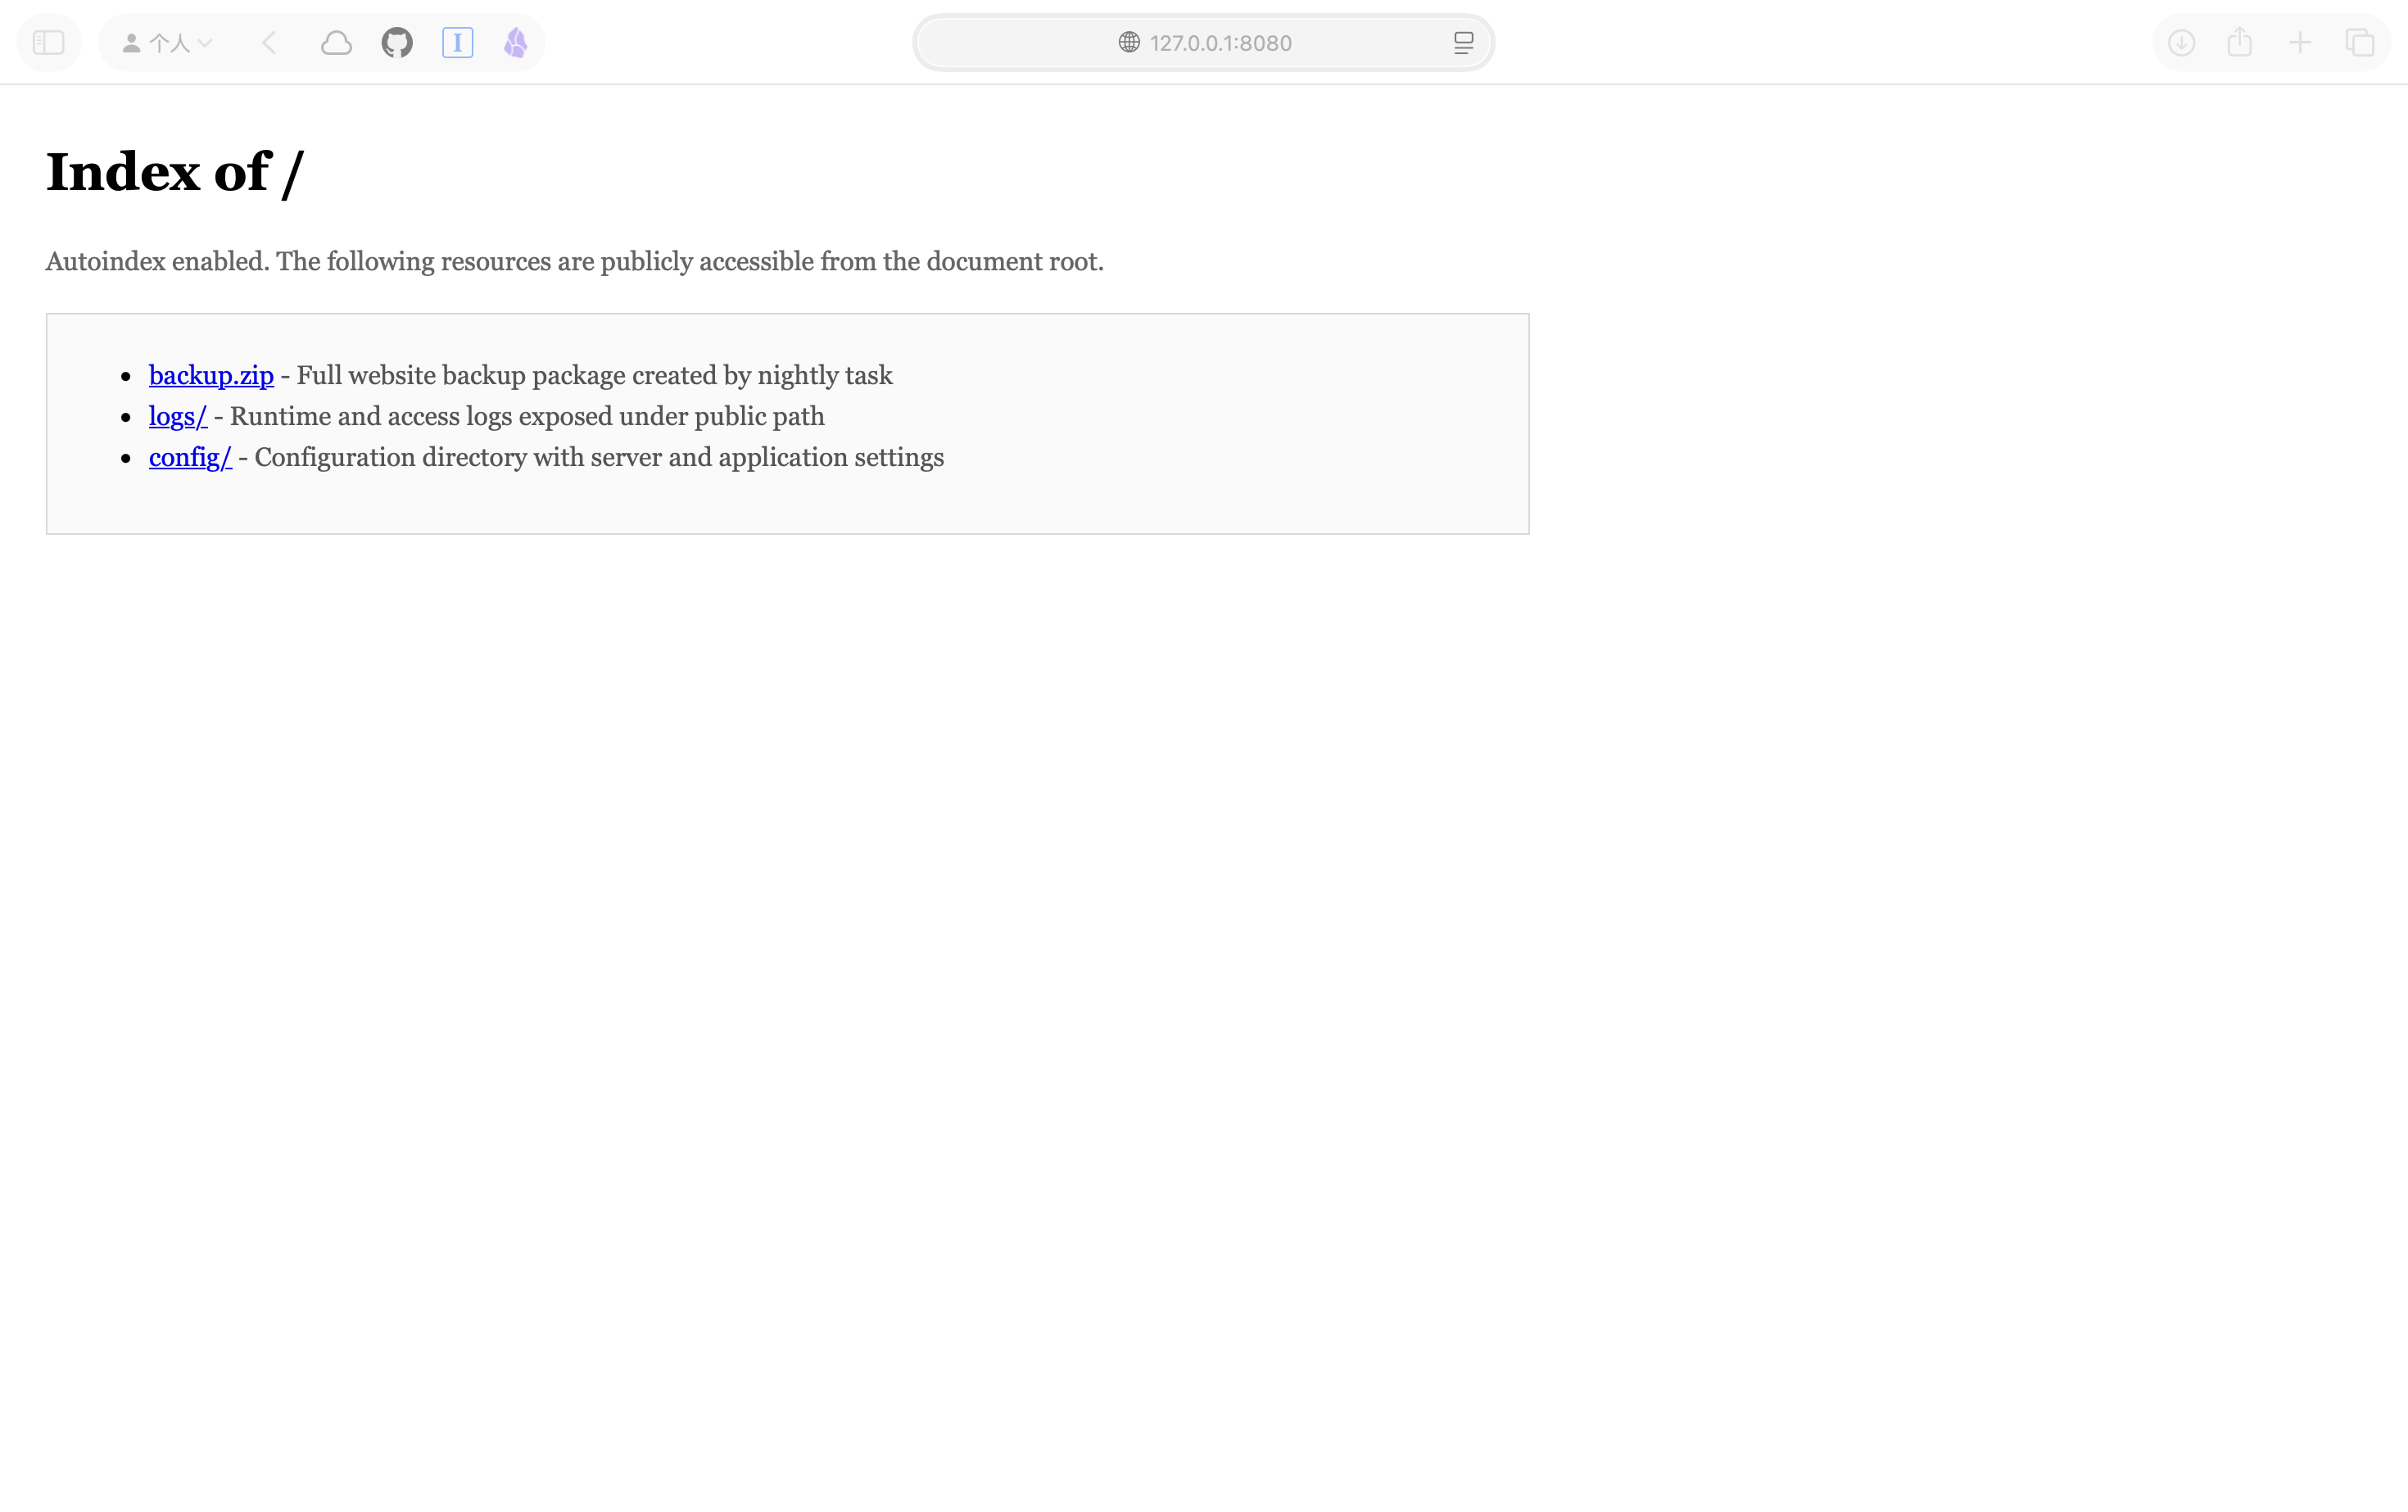
\includegraphics[width=0.95\textwidth]{figures/demo_site_screenshot.png}
  \caption{本地弱配置演示服务页面截图（目录索引暴露场景）}
  \label{fig:directory-screenshot}
\end{figure}

图 \ref{fig:directory-screenshot} 展示了本地弱配置演示服务的真实页面，可以看到浏览器列出了 \texttt{backup.zip}、\texttt{logs/}、\texttt{config/} 等目录内容，页面底部显示了 \texttt{Apache/2.4.49} 版本信息。这两项证据直接对应了检测系统识别出的“目录索引暴露”与“Server 版本信息暴露”两个风险项。

\section{实验设计与执行结果}

\subsection{实验环境与整体流程}

实验以本地回环地址 \texttt{127.0.0.1} 为扫描目标。首先启动弱配置演示服务，随后调用主扫描程序对 80、443 和 8080 端口进行检测。实验步骤如下：

\begin{enumerate}[label=\arabic*.]
  \item 启动本地演示服务：
\begin{lstlisting}[language=bash]
python3 demo_vulnerable_server.py
\end{lstlisting}
  \item 运行风险扫描程序：
\begin{lstlisting}[language=bash]
python3 risk_scanner.py --host 127.0.0.1 --ports 80,443,8080 --output-dir results/exp1
\end{lstlisting}
\end{enumerate}

本实验对应的完整输出文件保存在 \texttt{results/exp1/} 目录中（\texttt{scan\_result.json} 与 \texttt{scan\_report.md}），后续三组实验的输出分别保存于 \texttt{results/exp2}、\texttt{results/exp3} 与 \texttt{results/exp4} 目录，便于按实验编号独立查阅与复现，避免相互覆盖。

\begin{figure}[H]
  \centering
  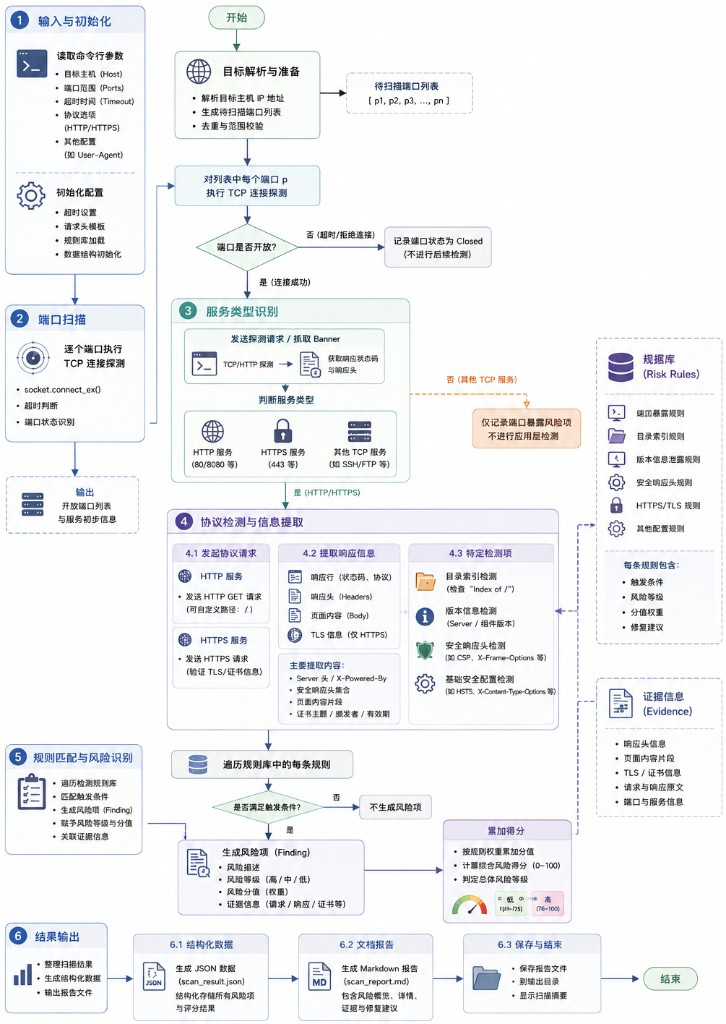
\includegraphics[width=0.95\textwidth]{figures/workflow.png}
  \caption{系统工作流程图}
  \label{fig:workflow}
\end{figure}

图 \ref{fig:workflow} 描述了系统从输入与初始化、端口扫描、服务类型识别、协议检测与信息提取、规则匹配与风险识别到结果输出的完整工作流程，有助于阅读者把握系统运行路径与各阶段的判定逻辑。

\subsection{实验一：基础端口扫描}

\begin{table}[H]
  \centering
  \caption{端口扫描结果}
  \begin{tabularx}{\textwidth}{>{\centering\arraybackslash}p{2cm} >{\centering\arraybackslash}p{2.2cm} >{\centering\arraybackslash}p{2.5cm} X}
    \toprule
    端口 & 状态 & 服务类型 & 说明 \\
    \midrule
    80 & closed & HTTP & 当前未启用明文 Web 服务 \\
    443 & closed & HTTPS & 当前未启用 HTTPS 服务 \\
    8080 & open & HTTP-Alt & 本地演示弱安全配置服务处于开放状态 \\
    \bottomrule
  \end{tabularx}
\end{table}

\subsection{实验一：基础风险检测}

实验结果表明，系统共识别出 8 个风险项，其中高风险 1 项、中风险 5 项、低风险 2 项，综合风险评分为 76，总体等级为中风险。具体结果如表 \ref{tab:risk-summary} 所示。

\begin{table}[H]
  \centering
  \caption{风险检测结果汇总}
  \label{tab:risk-summary}
  \begin{tabularx}{\textwidth}{>{\centering\arraybackslash}p{0.9cm} X >{\centering\arraybackslash}p{1.8cm} >{\centering\arraybackslash}p{1.4cm}}
    \toprule
    序号 & 风险项 & 严重级别 & 分值 \\
    \midrule
    1 & 疑似目录索引暴露 & 高风险 & 20 \\
    2 & 开放端口 8080 暴露风险 & 中风险 & 10 \\
    3 & 缺少 Strict-Transport-Security & 中风险 & 10 \\
    4 & 缺少 Content-Security-Policy & 中风险 & 10 \\
    5 & Server 版本信息暴露 & 中风险 & 8 \\
    6 & 缺少 X-Frame-Options & 中风险 & 8 \\
    7 & 缺少 X-Content-Type-Options & 低风险 & 6 \\
    8 & 缺少 Referrer-Policy & 低风险 & 4 \\
    \bottomrule
  \end{tabularx}
\end{table}

\begin{figure}[H]
  \centering
  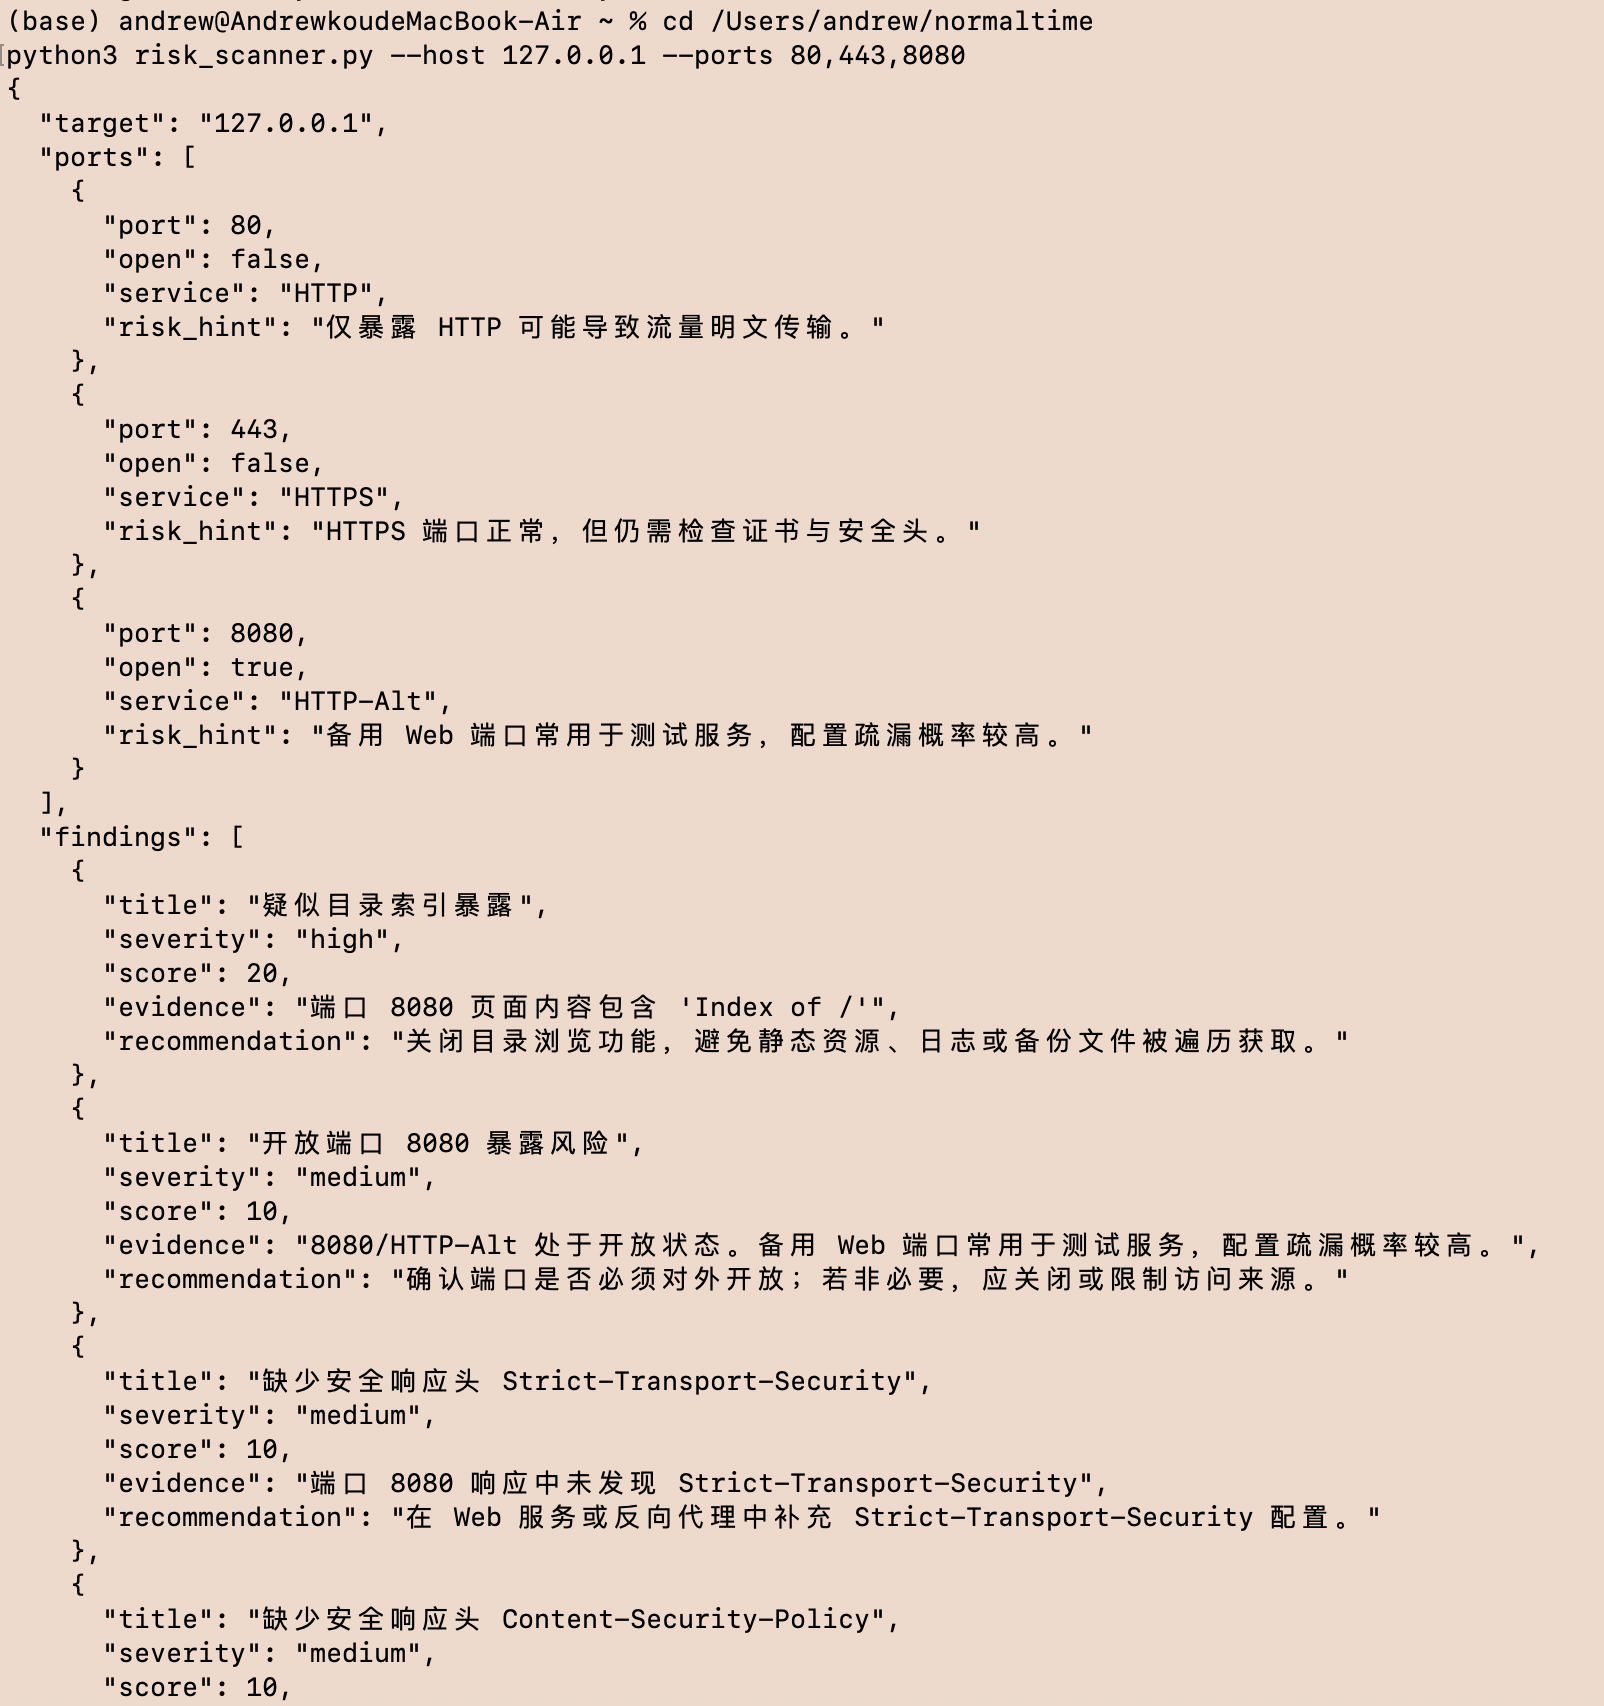
\includegraphics[width=0.95\textwidth]{figures/terminal_output_1.png}
  \caption{风险扫描程序运行结果（终端输出上半部分：端口扫描与前四项风险）}
  \label{fig:terminal-output}
\end{figure}

\begin{figure}[H]
  \centering
  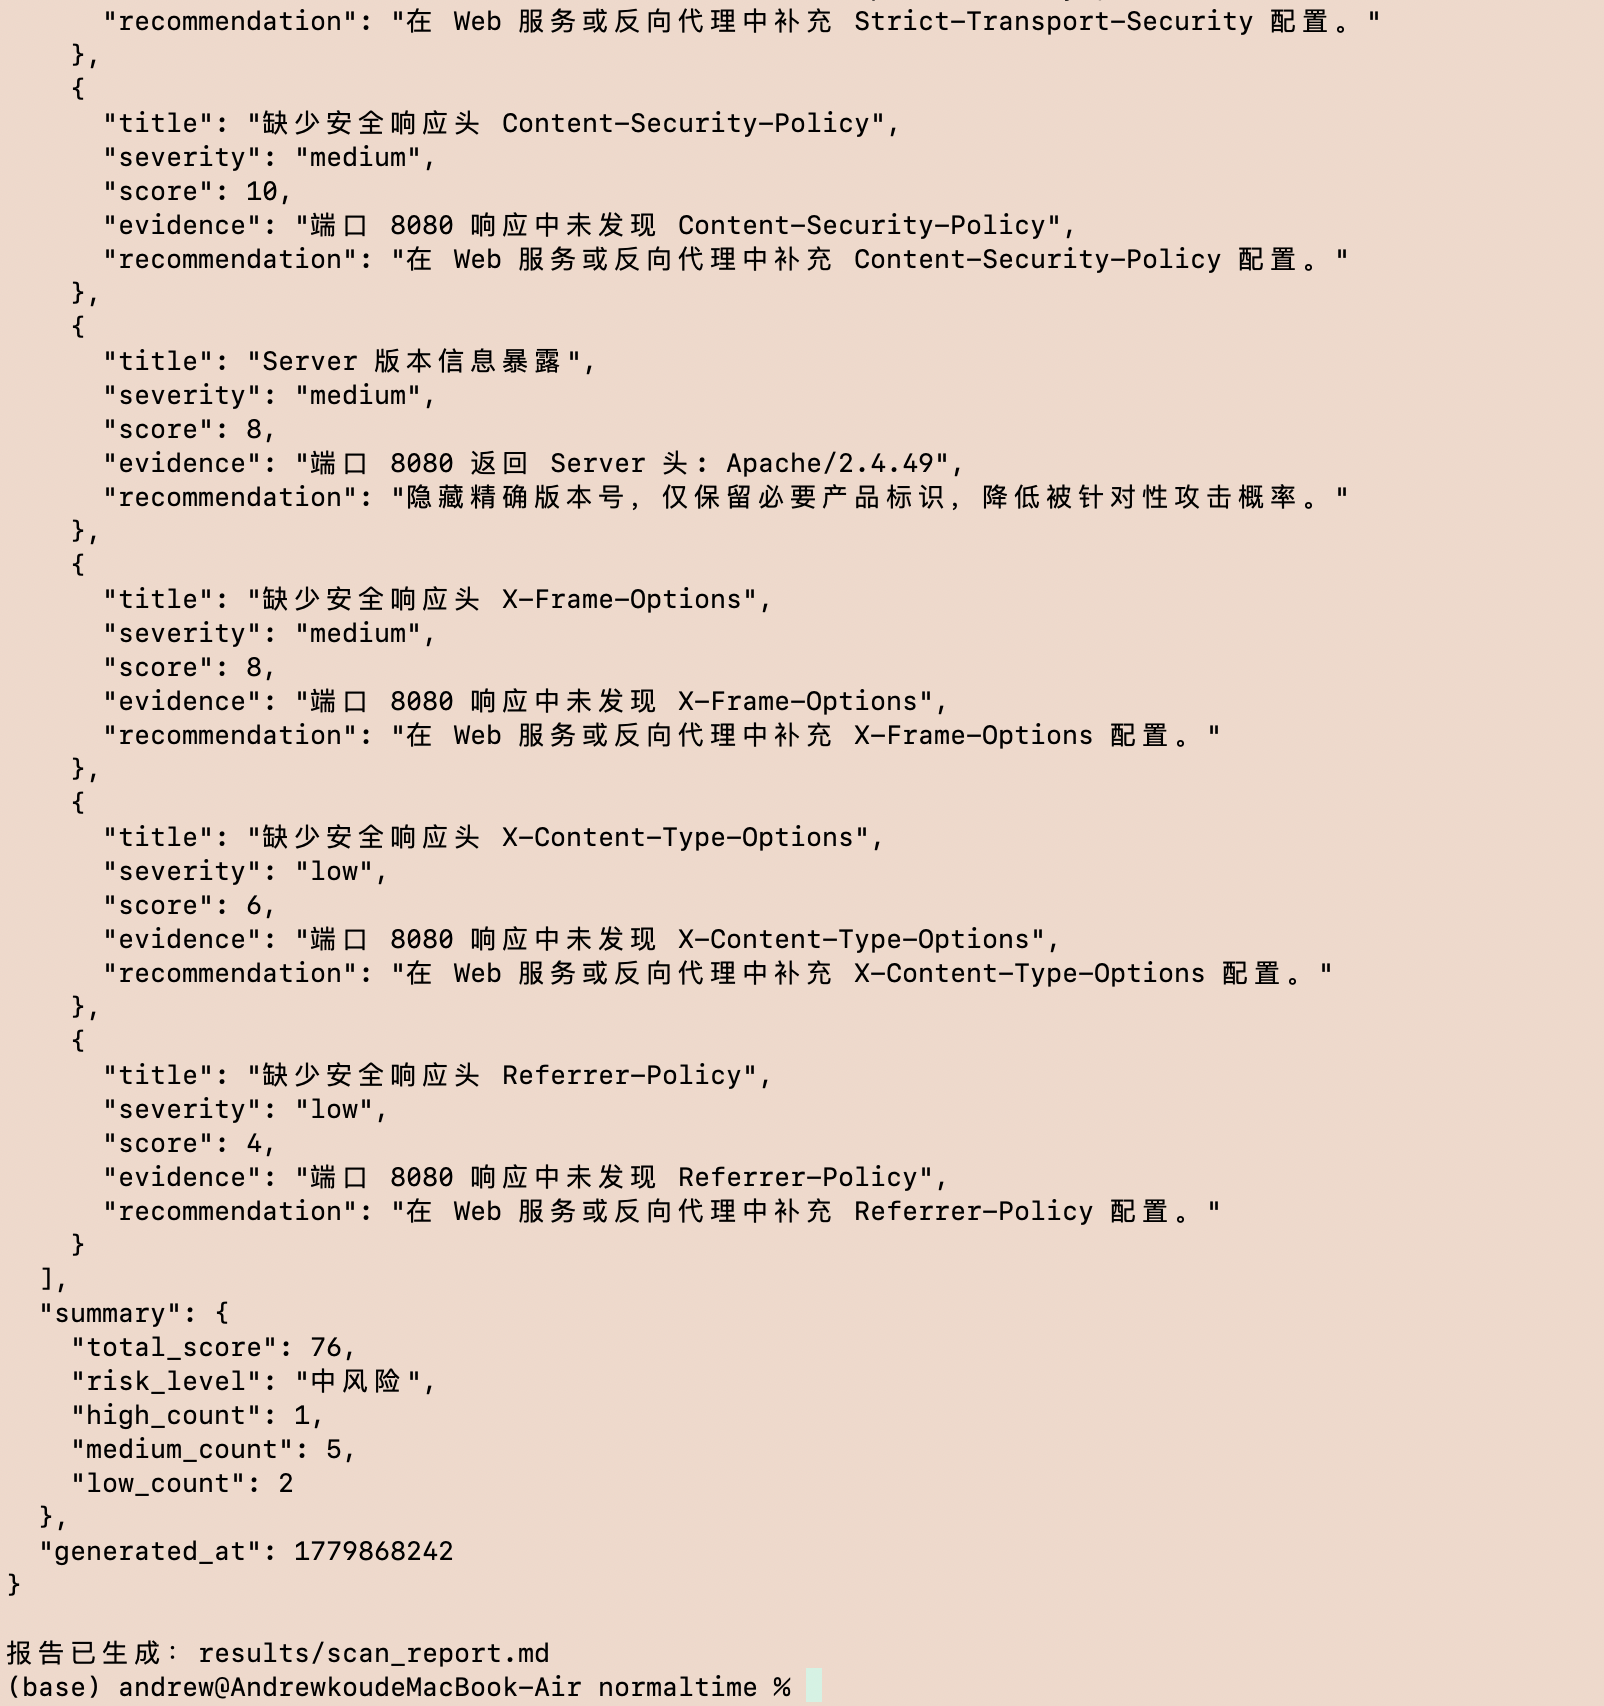
\includegraphics[width=0.95\textwidth]{figures/terminal_output_2.png}
  \caption{风险扫描程序运行结果（终端输出下半部分：剩余风险项与综合评分）}
  \label{fig:terminal-output2}
\end{figure}

\begin{figure}[H]
  \centering
  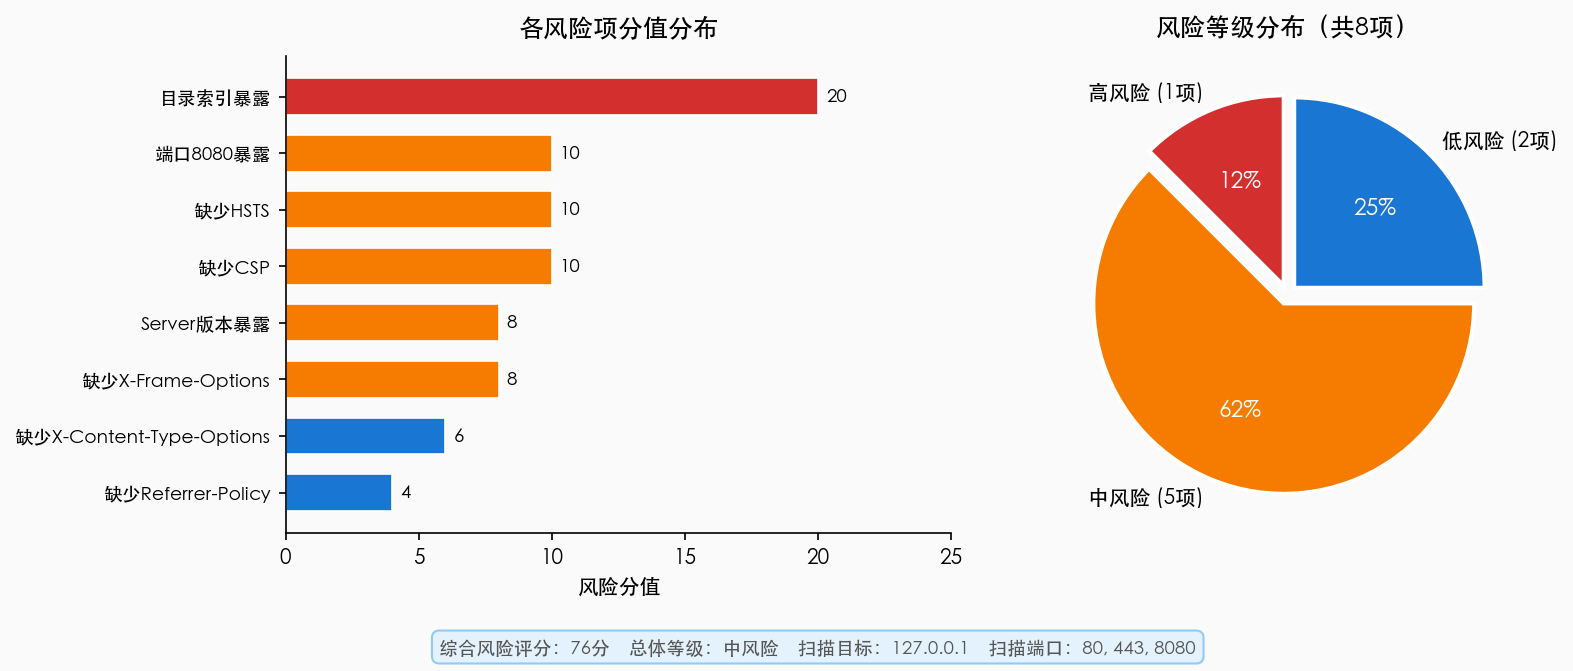
\includegraphics[width=0.95\textwidth]{figures/risk_chart.png}
  \caption{风险统计图（各风险项分值分布与严重级别占比）}
  \label{fig:risk-chart}
\end{figure}

\subsection{实验一：结果分析}

从端口结果看，目标主机仅在 8080 端口上对外提供可访问服务，这说明系统能够准确识别实验环境中的暴露入口。从风险结果看，检测系统并未止步于“端口开放”这一表层事实，而是进一步识别出目录索引暴露、版本信息泄露和多项安全响应头缺失等典型问题，说明系统已经具备了由连接性检测向配置性分析延伸的能力。

综合得分 76 被系统判定为中风险，这一结果与实验场景基本一致。尽管演示服务并未模拟认证缺失、远程命令执行等更严重问题，但其暴露出的多项基础弱配置已经足以构成真实环境中的安全隐患。尤其是目录索引暴露和版本信息暴露，往往会成为攻击者建立后续攻击路径的重要前置条件。

若从防守者的视角进一步分析，本系统输出的风险结果还具有一定的优先级指导意义。例如，在 8 个风险项中，“目录索引暴露”和“测试端口暴露”应优先整改，因为它们直接关系到暴露面的存在及敏感资源被枚举的可能性；“安全响应头缺失”虽更多属于浏览器侧防护不足问题，但若长期忽视，则会在系统面对复杂攻击链时进一步放大风险。也就是说，本文的结果不仅能说明“系统存在问题”，还能够支持“问题先后怎么处理”的基本决策。

从风险分析完整性的角度看，这一点同样重要。仅展示程序能够运行并不足以说明系统具备安全分析价值，本文更强调从输出结果中进一步解释系统状态、识别风险类别并形成整改优先级，使执行结果能够转化为可讨论、可复核、可处置的风险结论，而不只是编程功能的演示。

\subsection{实验二：扩大端口范围扫描}

为验证系统对多类敏感端口的综合识别能力，本文额外设计了一组扩展扫描实验，将扫描端口范围扩展至 21（FTP）、22（SSH）、23（Telnet）、80（HTTP）、443（HTTPS）、3306（MySQL）、6379（Redis）和 8080（HTTP-Alt）共 8 个端口，同样以本地 \texttt{127.0.0.1} 为目标。

\begin{lstlisting}[language=bash]
python3 risk_scanner.py --host 127.0.0.1 --ports 21,22,23,80,443,3306,6379,8080 --output-dir results/exp2
\end{lstlisting}

实验结果显示，在扩展端口列表中，系统识别出 22 端口（SSH）处于开放状态。由于端口 22 在当前预设字典中被标记为未知服务（宿主机 SSH 服务在运行），系统对其给出了"未知服务、请结合实际业务研判"的风险提示，并按默认分值计入综合评分。本次实验共识别出 9 个风险项，综合风险评分上升至 81 分，系统将整体等级由上一实验的"中风险"升级为"\textbf{高风险}"。具体结果如表 \ref{tab:extend-risk} 所示，完整输出见 \texttt{results/exp2/scan\_result.json} 与 \texttt{results/exp2/scan\_report.md}。

\begin{table}[H]
  \centering
  \caption{扩展端口扫描风险结果汇总}
  \label{tab:extend-risk}
  \begin{tabularx}{\textwidth}{>{\centering\arraybackslash}p{0.9cm} X >{\centering\arraybackslash}p{1.8cm} >{\centering\arraybackslash}p{1.4cm}}
    \toprule
    序号 & 风险项 & 严重级别 & 分值 \\
    \midrule
    1 & 疑似目录索引暴露 & 高风险 & 20 \\
    2 & 开放端口 8080 暴露风险 & 中风险 & 10 \\
    3 & 缺少 Strict-Transport-Security & 中风险 & 10 \\
    4 & 缺少 Content-Security-Policy & 中风险 & 10 \\
    5 & Server 版本信息暴露 & 中风险 & 8 \\
    6 & 缺少 X-Frame-Options & 中风险 & 8 \\
    7 & 缺少 X-Content-Type-Options & 低风险 & 6 \\
    8 & 开放端口 22 暴露风险 & 中风险 & 5 \\
    9 & 缺少 Referrer-Policy & 低风险 & 4 \\
    \bottomrule
  \end{tabularx}
\end{table}

该实验说明系统能够随端口范围的扩大动态调整风险识别结果，并相应提升综合评分与整体等级判定。尤其是端口 22 的识别体现了系统对常见服务端口的覆盖能力：即使当前知识库尚未对 SSH 服务做深度分析，仍能标记其开放状态并给出基础风险提示，提醒运维人员关注。此外，本次实验总分达到 81 分，触发了算法中 $S \geq 80$ 的高风险判定条件，说明评分规则对累积风险具有合理的敏感性。

\subsection{实验三：无演示服务基线扫描}

为进一步验证系统的准确性，本文设计了一组对照实验：在未启动本地演示服务的情况下对同一目标（\texttt{127.0.0.1}，端口 80、443、8080）执行扫描，观察系统在"无已知风险"环境下的输出行为。

\begin{lstlisting}[language=bash]
python3 risk_scanner.py --host 127.0.0.1 --ports 80,443,8080 --output-dir results/exp3
\end{lstlisting}

实验结果显示，三个端口全部处于关闭状态，系统未发现任何 HTTP 或 HTTPS 服务，\texttt{findings} 列表为空，综合评分为 0，整体等级判定为"\textbf{低风险}"。完整输出见 \texttt{results/exp3/scan\_result.json} 与 \texttt{results/exp3/scan\_report.md}，核心结果如下：

\begin{lstlisting}[language=json]
{
  "target": "127.0.0.1",
  "findings": [],
  "summary": {
    "total_score": 0,
    "risk_level": "低风险",
    "high_count": 0,
    "medium_count": 0,
    "low_count": 0
  }
}
\end{lstlisting}

该结果证明系统具备正确的"无风险"识别能力，不会产生虚假告警（False Positive）。这一对照实验的意义在于：若系统在无实际风险的情况下仍输出大量告警，说明规则设计过于宽松；而本次实验结果表明，系统的检测逻辑与实际服务状态高度一致，仅在服务真实存在且配置存在问题时才会生成风险项。

\subsection{实验四：HTTPS 自签名证书检测}

前述三组实验中，443 端口始终处于关闭状态，4.6 节实现的 HTTPS 检测模块虽已完成编码，但未曾真正执行。为弥补这一空白，本文按照 4.10 节所述方式，为本地演示服务额外开启了一个基于自签名证书的 HTTPS 监听端口（8443），并以此为目标重新执行扫描，使 \texttt{check\_https\_service()} 的两阶段握手逻辑在真实 TLS 连接上得到验证。

\begin{enumerate}[label=\arabic*.]
  \item 启动本地演示服务（同时监听 8080/HTTP 与 8443/HTTPS）：
\begin{lstlisting}[language=bash]
python3 demo_vulnerable_server.py
\end{lstlisting}
  \item 运行风险扫描程序，将 8443 纳入扫描端口范围：
\begin{lstlisting}[language=bash]
python3 risk_scanner.py --host 127.0.0.1 --ports 80,443,8080,8443 --output-dir results/exp4
\end{lstlisting}
\end{enumerate}

\begin{table}[H]
  \centering
  \caption{实验四端口扫描结果}
  \begin{tabularx}{\textwidth}{>{\centering\arraybackslash}p{2cm} >{\centering\arraybackslash}p{2.2cm} >{\centering\arraybackslash}p{2.5cm} X}
    \toprule
    端口 & 状态 & 服务类型 & 说明 \\
    \midrule
    80 & closed & HTTP & 当前未启用明文 Web 服务 \\
    443 & closed & HTTPS & 标准 HTTPS 端口未启用 \\
    8080 & open & HTTP-Alt & 本地演示弱安全配置服务处于开放状态 \\
    8443 & open & HTTPS-Alt & 本地自签名证书 HTTPS 演示服务处于开放状态 \\
    \bottomrule
  \end{tabularx}
\end{table}

实验结果显示，系统对 8443 端口的 HTTPS 检测按预期触发了 4.6 节描述的两阶段握手流程：第一阶段使用严格校验上下文 \texttt{ssl.\allowbreak create\_default\_context()} 握手时，因证书的颁发者与使用者相同而抛出异常 \texttt{ssl.\allowbreak SSLCertVerificationError}，OpenSSL 返回 \texttt{verify\_code=18}、\texttt{verify\_message=}\allowbreak\texttt{"self-signed certificate"}；系统据此生成"HTTPS 证书为自签名证书"风险项（中风险，12 分）。随后第二阶段使用 \texttt{verify\_mode=}\allowbreak\texttt{ssl.CERT\_NONE} 的非校验上下文重新握手成功，得到协商结果为 \texttt{TLSv1.3} 与密码套件 \texttt{TLS\_AES\_256\_\allowbreak GCM\_SHA384}——均为当前推荐的安全配置，因此 TLS 协议版本检查与弱密码套件检查均未产生额外风险项。本次实验连同 8080 端口的既有风险项，系统共识别出 9 个风险项，综合风险评分上升至 \textbf{88} 分，整体等级判定为"\textbf{高风险}"。具体结果如表 \ref{tab:exp4-risk} 所示，完整输出见 \texttt{results/exp4/\allowbreak scan\_result.json} 与 \texttt{results/exp4/\allowbreak scan\_report.md}。

\begin{table}[H]
  \centering
  \caption{实验四风险检测结果汇总}
  \label{tab:exp4-risk}
  \begin{tabularx}{\textwidth}{>{\centering\arraybackslash}p{0.9cm} X >{\centering\arraybackslash}p{1.8cm} >{\centering\arraybackslash}p{1.4cm}}
    \toprule
    序号 & 风险项 & 严重级别 & 分值 \\
    \midrule
    1 & 疑似目录索引暴露 & 高风险 & 20 \\
    2 & HTTPS 证书为自签名证书 & 中风险 & 12 \\
    3 & 开放端口 8080 暴露风险 & 中风险 & 10 \\
    4 & 缺少 Strict-Transport-Security & 中风险 & 10 \\
    5 & 缺少 Content-Security-Policy & 中风险 & 10 \\
    6 & Server 版本信息暴露 & 中风险 & 8 \\
    7 & 缺少 X-Frame-Options & 中风险 & 8 \\
    8 & 缺少 X-Content-Type-Options & 低风险 & 6 \\
    9 & 缺少 Referrer-Policy & 低风险 & 4 \\
    \bottomrule
  \end{tabularx}
\end{table}

该实验具有两方面意义。第一，它使 4.6 节实现的 HTTPS 检测代码不再是"未被执行的代码"，而是产生了真实、可复核的风险项，证据链中的 \texttt{verify\_code} 与 \texttt{verify\_message} 均直接来自 OpenSSL 的证书校验结果，具有较强的可信度。第二，TLS 协议版本与密码套件检查虽未触发风险项，但这本身也是一项有效验证：它说明系统在面对"协议配置安全、仅证书不受信任"的真实场景时，不会因为证书问题而错误地将协议版本或密码套件标记为风险，体现了规则判定的精确性。

需要说明的是，本次实验中证书有效期检查未被实际触发——这是因为第二阶段采用 \texttt{verify\_mode=ssl.CERT\_NONE} 进行非校验握手时，标准库 \texttt{getpeercert()} 按设计返回空字典，因此无法读取 \texttt{notAfter} 字段。这是 4.6 节已说明的一项已知边界：证书有效期检查仅在第一阶段握手即直接成功（即证书本身可信）时才会执行。该边界并不影响本次实验对"自签名证书识别"这一核心目标的验证，但作为系统的诚实局限性记录于此，并将在第 9 章的改进方向中一并讨论。

\subsection{四组实验对比分析}

综合四组实验结果，可以得出以下对比结论，如表 \ref{tab:exp-compare} 所示。

\begin{table}[H]
  \centering
  \caption{四组实验结果对比}
  \label{tab:exp-compare}
  \begin{tabularx}{\textwidth}{>{\centering\arraybackslash}p{0.7cm} X >{\centering\arraybackslash}p{1.6cm} >{\centering\arraybackslash}p{1.4cm} >{\centering\arraybackslash}p{1.8cm}}
    \toprule
    编号 & 实验场景 & 开放端口 & 综合评分 & 风险等级 \\
    \midrule
    1 & 基础扫描（80/443/8080，含演示服务） & 8080 & 76 & 中风险 \\
    2 & 扩展扫描（8端口，含演示服务） & 8080、22 & 81 & 高风险 \\
    3 & 基线扫描（80/443/8080，无服务） & 无 & 0 & 低风险 \\
    4 & HTTPS 自签名证书检测（80/443/8080/8443，含演示服务） & 8080、8443 & 88 & 高风险 \\
    \bottomrule
  \end{tabularx}
\end{table}

四组实验覆盖了低、中、高三个风险等级，验证了系统的评分模型能够随实际检测结果动态变化，不存在固定输出偏差。实验一与实验三的对比说明系统具有较好的检测精度；实验一与实验二的对比说明扩大扫描范围能够发现更多潜在风险；实验一与实验四的对比则进一步说明，在端口暴露面与 HTTP 配置问题不变的前提下，新增一个证书不受信任的 HTTPS 端口会使综合评分由 76 升至 88，并使风险等级由中风险升级为高风险，这与"自签名证书"在真实环境中通常被视为需要尽快处理的中高优先级问题这一安全直觉相符。四组实验共同表明，4.6 节实现的 HTTP 与 HTTPS 检测模块均已在真实场景下产生过可验证的输出，系统的代码开发、执行结果与风险展示三个环节不存在未经验证的"空模块"。

\section{风险展示}

\subsection{风险对象}

本次检测研究的是本地网络资产与 Web 服务基础安全配置中的五类典型风险。第一类是端口暴露风险，表现为目标主机对外开放 8080 测试端口，属于网络暴露面管理类风险。第二类是目录索引暴露风险，表现为 Web 服务器启用目录浏览功能，使外部访问者能够直接枚举服务器文件结构。第三类是服务版本信息泄露风险，表现为 \texttt{Server} 响应头返回精确的软件版本号，属于信息泄露类风险。第四类是安全响应头缺失风险，表现为 HTTP 响应未包含 HSTS、CSP 等浏览器侧安全响应头，属于协议配置类风险。第五类是 HTTPS 证书可信性风险，表现为 HTTPS 服务使用自签名证书，客户端无法通过默认信任链验证服务端身份，属于传输层身份验证类风险。

上述风险均属于基础安全配置层面的问题，其共同特点是检测门槛低、危害链条长，是攻击者实施信息收集和后续攻击的常见前置条件。其中前四类风险在实验一（5.2--5.4 节）中被同时观测到，第五类风险则在实验四（5.7 节）的本地自签名证书 HTTPS 演示环境中被独立验证。

\subsection{触发条件}

从触发条件看，第一，端口 8080 暴露的直接原因是本地弱配置演示服务主动监听该端口，并且没有配置防火墙规则或访问控制列表进行限制，导致扫描程序能够从目标地址直接建立 TCP 连接。第二，目录索引暴露的触发条件是 Web 服务器的目录浏览功能处于启用状态，同时请求路径下不存在默认索引文件，例如 \texttt{index.html}，服务器因而返回目录列表页面。第三，服务版本信息泄露的触发条件是 Web 服务器未隐藏版本号，例如未采用 Apache 的 \texttt{ServerTokens Prod}、\texttt{ServerSignature Off} 或 Nginx 的 \texttt{server\_tokens off} 等配置，使 \texttt{Server} 响应头直接暴露组件名称与精确版本。第四，安全响应头缺失的触发条件是 Web 应用或前置反向代理没有在响应中追加 HSTS、CSP、X-Frame-Options 等安全头，导致浏览器侧缺乏必要的行为约束与防护指令。第五，HTTPS 证书不受信任的触发条件是服务部署时使用自签名证书，证书的颁发者与使用者相同，且未接入受信任的公共或私有证书颁发机构，因此客户端默认证书校验流程无法建立信任链。

\subsection{风险证据}

扫描程序在本次实验中采集到的证据可以从六个方面说明。第一，在端口开放证据上，程序对 8080 端口执行 TCP 连接尝试，\texttt{socket.connect\_ex()} 返回值为 0，确认该端口处于开放状态。第二，在目录索引证据上，程序对 \texttt{http://127.0.0.1:8080/} 发起 GET 请求，响应正文包含特征字符串 \texttt{Index of /}，并列出了 \texttt{backup.zip}、\texttt{logs/}、\texttt{config/} 等路径，因此触发目录索引暴露风险项，风险分值为 20。第三，在版本信息证据上，HTTP 响应头中的 \texttt{Server} 字段值为 \texttt{Apache/2.4.49}，程序判断其包含精确版本号，因而触发版本信息暴露风险项，风险分值为 8。第四，在安全响应头证据上，程序遍历预设安全响应头集合，确认 \texttt{Strict-Transport-Security}、\texttt{Content-Security-Policy}、\texttt{X-Frame-Options}、\texttt{X-Content-Type-Options} 和 \texttt{Referrer-Policy} 均未在响应中出现，对应分值分别为 10、10、8、6 和 4。第五，在 HTTPS 证书可信性证据上，实验四中程序对 \texttt{127.0.0.1:8443} 发起 TLS 握手，使用严格校验上下文 \texttt{ssl.\allowbreak create\_default\_context()} 时抛出 \texttt{ssl.\allowbreak SSLCertVerificationError}，OpenSSL 返回 \texttt{verify\_code=18}、\texttt{verify\_message=}\allowbreak\texttt{"self-signed certificate"}，因此触发“HTTPS 证书为自签名证书”风险项，风险分值为 12。第六，在综合风险分值上，实验一场景下累计风险总分为 76 分，其中高风险项 1 个、中风险项 5 个、低风险项 2 个，终端输出与 JSON 报告均记录了上述结果；在叠加 HTTPS 自签名证书风险的实验四场景下，综合风险总分上升至 88 分，整体等级由中风险升级为高风险，具体结果见表 \ref{tab:exp4-risk}。

\subsection{影响分析}

针对上述风险，其影响范围与危害程度可以从五个层面分析。第一，测试端口长期对外开放意味着该服务可被任意来源访问，而测试服务通常比正式主站配置更弱，容易遗留调试接口、默认路径或默认凭据。一旦该端口与弱口令、未授权访问漏洞或后台接口暴露叠加，就可能成为横向移动入口，因此系统将 8080 端口暴露评为中风险。

第二，目录索引暴露会直接破坏服务器文件结构的保密性。攻击者无需认证即可枚举目录内容，若目录中存在备份压缩包、日志文件或配置文件，就可能进一步泄露数据库密码、API 密钥、用户数据和服务拓扑。本例中页面列出了 \texttt{backup.zip}、\texttt{logs/} 和 \texttt{config/} 等路径，敏感程度较高，因此系统将该项判定为高风险，分值为 20。

第三，服务版本信息泄露本身看似只是细节暴露，但会显著降低漏洞匹配成本。本次实验检测到 \texttt{Server} 头返回 \texttt{Apache/2.4.49}。需要说明的是，本地演示服务由 Python \texttt{http.server} 模拟实现，仅将该字符串写入 \texttt{Server} 响应头以复现“版本信息泄露”这一现象，并未真实运行 Apache 2.4.49，因此本次实验本身不构成对具体 CVE 的复现或利用验证。不过，该字符串对应的真实软件版本确实存在被广泛利用的高危漏洞。例如，CVE-2021-41773 属于路径穿越与远程代码执行漏洞，CVSS v3.1 评分为 7.5；CVE-2021-42013 则是 CVE-2021-41773 的绕过变体，CVSS v3.1 评分达到 9.8。二者说明，一旦真实环境中存在相同版本且未修补，攻击者仅凭版本号就可能在公开漏洞库中快速匹配利用脚本。这正是版本信息泄露被列为风险项的根本原因。本次实验中该项严重程度评为中风险，分值为 8。

第四，安全响应头缺失会削弱浏览器侧的多层防护能力。缺少 HSTS 时，浏览器无法强制使用 HTTPS，攻击者可能通过降级攻击将连接诱导到明文 HTTP；缺少 CSP 时，页面资源加载来源缺乏限制，一旦存在 XSS 注入点，恶意脚本更容易执行；缺少 X-Frame-Options 或等价的 \texttt{frame-ancestors} 策略时，页面可能被嵌入恶意框架并触发点击劫持；缺少 X-Content-Type-Options 时，浏览器 MIME 嗅探行为可能导致伪装资源被当作脚本执行；缺少 Referrer-Policy 时，页面跳转过程中可能泄露敏感路径。多个头部同时缺失会形成叠加效应，使系统面对复合型攻击时防护能力明显下降。

第五，HTTPS 证书可信性风险直接影响传输层身份验证。自签名证书意味着客户端无法通过公认信任链验证服务端身份，攻击者有机会在网络路径中插入伪造证书并实施中间人攻击。在生产环境中，自签名证书还可能导致依赖严格证书校验的客户端、API 调用方或自动化脚本直接连接失败，影响业务可用性。本次实验中该项严重程度评为中风险，分值为 12；若该端口实际承载身份认证或敏感数据传输业务，其现实风险等级还应结合业务重要性进一步上调。

\subsection{展示结论}

综合以上风险对象、触发条件、证据与影响分析，系统对目标主机 \texttt{127.0.0.1} 的基础场景（实验一）风险等级判定为\textbf{中风险}，综合评分为 76 分。该结论主要来自三个方面：第一，系统识别出 1 个高风险项，即目录索引暴露，分值为 20，直接威胁服务器文件保密性；第二，系统识别出 5 个中风险项，包括端口暴露、HSTS 缺失、CSP 缺失、版本泄露和 X-Frame-Options 缺失，合计 46 分，说明目标服务存在多维度防护短板；第三，系统还识别出 2 个低风险项，即 X-Content-Type-Options 缺失和 Referrer-Policy 缺失，合计 10 分，属于浏览器侧附加防护不足。按照系统评分规则，总分 $S = 76 \geq 40$，且存在高风险项 $H = 1 \geq 1$，因此基础场景最终等级定为\textbf{中风险}。

在此基础上，实验四进一步引入了 HTTPS 证书可信性风险：当目标主机额外开放一个使用自签名证书的 HTTPS 端口（8443）时，系统新增"HTTPS 证书为自签名证书"风险项（中风险，12 分），综合评分由 76 分上升至 88 分，触发系统评分规则中"总分 $S \geq 80$"的条件，整体等级由中风险升级为\textbf{高风险}。这一变化直接体现了风险评分模型对新增风险项的敏感性，也说明 HTTPS 层面的配置问题（即便协议版本和密码套件均符合现代安全标准）同样可以成为压垮整体风险等级的"最后一根稻草"。

需要说明的是，本次实验基于本地构造的弱配置演示环境，场景可控、结果可复现，但与真实生产网络相比，真实环境中往往还伴随更复杂的访问控制策略、代理转发链路和业务敏感性差异。因此，本系统更适合定位为基础风险巡检原型与可解释检测工具，后续可通过引入资产重要度权重、弱口令检测和漏洞情报关联等能力进一步完善。

\section{算法设计与复杂度分析}

\subsection{算法设计思想}

从更抽象的角度看，本文系统可以视为一个面向安全状态识别的规则驱动算法框架。其核心不是依赖复杂机器学习模型，而是依赖“输入采集一特征提取一规则映射一风险量化”的处理链。对于本文场景而言，这种方法具有两个优势：第一，逻辑透明，便于解释每一步为什么这样做；第二，便于验证，能够清晰观察输入变化如何影响最终输出。

尤其在网络安全基础巡检场景中，许多问题本身就适合用规则表示。例如，“响应中缺少某安全头”本质上是布尔判定问题，“页面正文包含目录索引特征”本质上是字符串匹配问题，“证书剩余有效期低于阈值”本质上是阈值比较问题。将这些问题形式化之后，便可以自然地组织为一组简洁但有效的检测算法。

\subsection{时间复杂度分析}

设待扫描端口数量为 $m$，每个开放 Web 端口所需执行的 HTTP 或 HTTPS 检查规则数量分别为 $h$ 和 $s$。则系统整体时间开销主要由三部分构成：

\begin{enumerate}[label=\arabic*.]
  \item 端口扫描阶段：对每个端口执行一次连接尝试，时间复杂度可近似视为 $O(m)$；
  \item HTTP/HTTPS 检测阶段：对开放服务执行规则匹配，若开放端口数量为 $k$，则额外复杂度约为 $O(k(h+s))$；
  \item 报告生成阶段：对全部风险项进行排序与输出，若风险项数量为 $n$，则复杂度约为 $O(n \log n)$。
\end{enumerate}

因此，系统总体复杂度可以近似表达为：

\begin{equation}
T(m, k, n) = O(m) + O(k(h+s)) + O(n \log n)
\end{equation}

在本文实验场景下，由于扫描端口数和风险项数量都相对有限，系统运行开销较低，能够满足快速验证和多次重复执行的需要。

\subsection{空间复杂度分析}

系统的空间开销主要来自端口结果集合与风险项集合的存储。若端口数量为 $m$，风险项数量为 $n$，则空间复杂度可近似记为：

\begin{equation}
S(m, n) = O(m+n)
\end{equation}

由于结果对象结构较为轻量，且实验中主机数量有限，因此空间开销在普通个人计算环境中可以忽略不计。这也说明本文方法非常适合作为本地化巡检原型或轻量级安全基线检测系统。

\subsection{与传统人工巡检方式的比较}

若采用人工巡检方式，安全检查人员需要逐个确认端口开放情况、访问页面查看响应头、检查目录是否暴露，并结合经验总结问题。这种方式虽然灵活，但存在效率低、重复劳动多、结果标准不统一等问题。相比之下，本文提出的方法能够将一组稳定的检查规则自动化执行，并统一生成结构化结果。尽管它暂时不能完全替代人工深度分析，但在基础巡检和初步筛查阶段已经具有明显优势。

\section{相关工作与技术对比}

\subsection{主流安全扫描工具概述}

在网络安全领域，已存在若干成熟的扫描与检测工具，它们从不同维度解决安全评估问题。本文在设计与实现过程中，对以下几类典型工具的功能范围、使用方式与局限性进行了分析，以明确本系统的定位与差异。

\textbf{（1）Nmap}

Nmap 是目前应用最广泛的开源网络扫描工具，支持主机发现、端口扫描、服务版本识别与操作系统指纹识别 \cite{nmap-book}。其核心优势在于扫描速度快、协议支持丰富，并可通过 NSE（Nmap Scripting Engine）脚本扩展检测能力。然而，Nmap 本质上是一个信息收集工具，其输出是原始的端口与服务状态，缺乏对 HTTP 安全响应头、目录索引暴露等 Web 层配置风险的结构化分析能力，也不具备风险评分与整改建议生成功能。

\textbf{（2）Nessus}

Nessus 是商业化的综合漏洞扫描平台，规则库涵盖数万条漏洞检测项，支持 CVSS 评分与合规报告输出 \cite{nessus-guide}。其优势在于覆盖面广、报告专业，但存在以下局限：其一，规则为封闭设计，使用者难以理解每条规则的判定逻辑；其二，部署成本高，需商业授权；其三，对于本文关注的可解释实现目标而言，过于完善的工具反而会掩盖检测原理，不利于展示风险识别的程序化过程。

\textbf{（3）OWASP ZAP}

OWASP ZAP（Zed Attack Proxy）是面向 Web 应用的开源安全测试工具，支持主动扫描、被动扫描与 API 安全测试 \cite{owasp-asvs}。其被动扫描功能可识别安全响应头缺失等问题，与本系统覆盖范围有一定重叠。然而，ZAP 以代理方式工作，需要浏览器或请求流量经过其代理端口，使用方式与本系统的命令行直接扫描有本质区别，且其输出缺乏针对特定端口暴露面的综合评分能力。

\textbf{（4）nikto}

nikto 是专注于 Web 服务器的开源扫描工具，能够检测过时软件版本、危险文件路径和错误配置项 \cite{owasp-cheatsheet}。与本系统相比，nikto 的检测逻辑依赖于规则文件（如 \texttt{db\_tests}），可扩展性较低，且不具备端口层面的暴露面分析与综合风险评分输出能力。

\subsection{本系统与主流工具的能力对比}

基于上述分析，本文将本系统与上述四类工具在关键维度上进行对比，如表 \ref{tab:tool-compare} 所示。

\begin{table}[H]
  \centering
  \caption{本系统与主流工具能力对比}
  \label{tab:tool-compare}
  \begin{tabularx}{\textwidth}{X >{\centering\arraybackslash}p{1.5cm} >{\centering\arraybackslash}p{1.5cm} >{\centering\arraybackslash}p{1.5cm} >{\centering\arraybackslash}p{1.5cm} >{\centering\arraybackslash}p{1.5cm}}
    \toprule
    能力维度 & 本系统 & Nmap & Nessus & ZAP & nikto \\
    \midrule
    端口开放检测 & $\checkmark$ & $\checkmark$ & $\checkmark$ & — & — \\
    HTTP 安全头检测 & $\checkmark$ & — & $\checkmark$ & $\checkmark$ & $\checkmark$ \\
    目录索引检测 & $\checkmark$ & — & $\checkmark$ & $\checkmark$ & $\checkmark$ \\
    版本信息识别 & $\checkmark$ & $\checkmark$ & $\checkmark$ & $\checkmark$ & $\checkmark$ \\
    综合风险评分输出 & $\checkmark$ & — & $\checkmark$ & — & — \\
    整改建议生成 & $\checkmark$ & — & $\checkmark$ & 部分 & — \\
    代码逻辑透明可读 & $\checkmark$ & $\checkmark$ & — & $\checkmark$ & $\checkmark$ \\
    仅依赖标准库 & $\checkmark$ & — & — & — & — \\
    无需安装/配置代理 & $\checkmark$ & $\checkmark$ & 部分 & — & $\checkmark$ \\
    开源/免费 & $\checkmark$ & $\checkmark$ & — & $\checkmark$ & $\checkmark$ \\
    \bottomrule
  \end{tabularx}
\end{table}

\subsection{本系统的定位与差异化分析}

从表 \ref{tab:tool-compare} 可以看出，本系统并不追求与 Nessus 等工业级产品在规则覆盖面上的竞争，而是在以下几个维度上形成差异化定位：

\begin{enumerate}[label=\arabic*.]
  \item \textbf{端到端透明性}：本系统从端口探测到风险评分的全部逻辑均由 Python 标准库实现，使用者可以直接阅读和修改每一条规则，理解每一项风险是如何被发现和评分的。这是 Nessus 等商业工具无法提供的；

  \item \textbf{综合评分与等级输出}：Nmap 和 nikto 提供的是原始扫描结果，不具备将多维度风险汇总为统一评分与等级的能力。本系统的评分模型虽然简洁，但能够为使用者提供"当前安全状态有多严重"的直接判断；

  \item \textbf{极低的运行门槛}：依赖 Python 标准库意味着系统可以在任何已安装 Python 3 的环境中直接运行，无需额外安装依赖包、数据库或代理服务，这在轻量化验证和快速原型场景中具有明显优势；

  \item \textbf{面向可复核报告的设计}：系统的 Markdown 报告输出与 JSON 结构化导出，专门围绕“代码可读、结果可展示、分析可解释”的目标设计，是上述工具未有意覆盖的场景。
\end{enumerate}

总体而言，本系统更适合定位为一个\textbf{可解释的轻量级安全基线检测原型}，其价值不在于替代成熟安全产品，而在于将风险发现过程透明化、可编程化，使安全检测的底层逻辑能够被直接审查和验证。

\section{预防措施与改进建议}

针对本文识别出的端口暴露、目录索引暴露、版本信息泄露、安全响应头缺失以及 HTTPS 证书可信性不足等问题，预防措施不能停留在“注意加固”的口号层面，而应当围绕暴露面收敛、Web 配置加固、敏感文件治理、版本管理、传输层安全加固和持续巡检形成闭环。以下建议分别从被测对象整改和检测系统改进两个层面展开。

\subsection{暴露面收敛与访问控制}

端口暴露是本次实验中最先被系统识别出的风险入口。对于 8080 这类常用于测试、管理或备用 Web 服务的端口，首先应确认其业务必要性。如果该端口仅用于本地调试或临时验证，应在验证结束后关闭服务进程，并从防火墙规则、反向代理配置和启动脚本中移除对应暴露入口。如果该端口确有长期运行需求，则应限制访问来源，例如仅允许内网网段、VPN 出口或堡垒机访问，避免将管理型或测试型服务直接暴露在不可控网络范围内。

在工程实践中，暴露面治理还应与资产清单结合。服务上线、迁移和下线时，应同步更新端口清单、责任人、用途说明和访问策略。本文程序当前能够识别端口是否开放，后续可以增加“端口用途白名单”机制：当某端口虽然开放但不在允许清单中时，系统直接将其标记为异常暴露，从而减少人工判断成本。

\subsection{目录索引与敏感文件治理}

目录索引暴露是本次检测中危害最直接的风险项。对于 Web 服务，应在服务器配置中关闭目录浏览功能。例如 Apache 可通过关闭 \texttt{Indexes} 选项避免目录列表输出，Nginx 可确保 \texttt{autoindex off}。与此同时，还应检查 Web 根目录中是否存在备份包、日志文件、配置文件、数据库导出文件等高敏感资源。即使目录索引被关闭，只要敏感文件路径可被猜测或被历史链接引用，仍然可能造成泄露。

本文实验页面中出现的 \texttt{backup.zip}、\texttt{logs/} 和 \texttt{config/} 具有明显的敏感资源特征。针对这类文件，应至少采取三类措施：第一，从公开目录中移除备份、日志和配置文件；第二，对必须保留的下载资源增加鉴权与审计；第三，在部署流水线中加入文件类型与路径检查，阻止 \texttt{.env}、\texttt{.sql}、\texttt{.bak}、\texttt{.zip}、\texttt{access.log} 等文件被误发布到 Web 根目录。后续系统也可以扩展路径探测规则，对常见敏感文件名进行低频、可控的验证。

\subsection{版本信息隐藏与补丁管理}

服务版本信息泄露本身未必直接造成入侵，但它会显著降低攻击者匹配漏洞的成本。本文检测到的 \texttt{Apache/2.4.49} 就是典型示例：版本号一旦暴露，攻击者可以迅速关联到公开漏洞、利用条件和补丁状态。预防该问题需要同时处理“隐藏信息”和“修复根因”两个层面。

在信息隐藏层面，应减少响应头、错误页和默认页面中的精确版本信息。例如 Apache 可配置 \texttt{ServerTokens Prod} 与 \texttt{ServerSignature Off}，Nginx 可配置 \texttt{server\_tokens off}。在根因修复层面，应建立组件版本台账，定期比对安全公告和漏洞库，确保 Web 服务器、运行时、中间件和依赖组件处于受支持版本。仅隐藏版本号不能替代补丁更新；它只能降低被动指纹识别效率，不能消除已存在漏洞。

\subsection{HTTP 安全响应头加固}

本次实验中缺失的五类安全响应头分别对应不同浏览器侧防护能力。针对 Strict-Transport-Security，应在正式 HTTPS 服务中配置合理的 \texttt{max-age}，并在确认全站 HTTPS 可用后逐步考虑 \texttt{includeSubDomains}。针对 Content-Security-Policy，应结合页面资源加载方式制定白名单策略，优先限制脚本来源、对象加载和内联脚本执行。针对 X-Frame-Options 或等价的 CSP \texttt{frame-ancestors} 指令，应明确页面是否允许被嵌入第三方站点。针对 X-Content-Type-Options，建议设置为 \texttt{nosniff}，减少 MIME 嗅探带来的脚本执行风险。针对 Referrer-Policy，可根据业务需要选择 \texttt{strict-origin-when-cross-origin} 等相对稳妥的策略。

需要注意的是，安全响应头并非越多越好，也不能脱离业务页面直接套用模板。过于严格的 CSP 可能导致页面脚本、图片或接口请求被阻断；过于宽松的策略又难以形成防护效果。因此，整改时应先在测试环境验证，再逐步上线到生产环境，并通过浏览器控制台、访问日志和自动化巡检结果确认策略是否生效。

\subsection{HTTPS 证书与传输层安全加固}

实验四识别出的“HTTPS 证书为自签名证书”风险项，本质上是身份验证层面的问题：客户端虽然能够与服务端建立加密通道，但无法确认通道另一端就是预期的服务。对于面向公网的服务，应使用受信任公共 CA（如 Let's Encrypt 等自动化证书颁发机构）签发的证书，并建立自动续期机制，避免因人工疏忽导致证书过期或长期使用临时证书。对于仅服务于内部系统的场景，推荐部署私有 CA，将私有根证书统一分发并安装至内部客户端、服务器和自动化脚本的信任库中，从而在不暴露公网的前提下，仍然获得“身份可验证”的加密通信。

除证书可信性外，4.6 节实现的 \texttt{check\_https\_service()} 还覆盖了 TLS 协议版本与密码套件检查，依据 TLS 1.3 规范 \cite{rfc8446} 与业界最佳实践 \cite{tls-bcp,mozilla-tls}，应停用 TLS 1.0/1.1 并禁用 RC4、3DES 等弱密码套件，仅保留 TLS 1.2 及以上版本与 AEAD 类密码套件。本次实验四中协商结果为 TLSv1.3 与 \texttt{TLS\_AES\_256\_GCM\_SHA384}，说明该项配置已符合现代安全基线，但这一结论仅在第一阶段握手失败、第二阶段非校验握手成功的前提下取得；对于证书有效期检查，由于非校验握手下 \texttt{getpeercert()} 无法返回解析后的证书字段，建议在生产环境中优先解决证书可信性问题，使第一阶段握手能够直接成功，从而让证书有效期检查在常规巡检中持续生效。

\subsection{持续巡检与处置闭环}

基础安全配置风险具有反复出现的特点，单次整改并不能保证长期安全。本文系统可进一步接入定时任务，在固定周期内对目标主机执行端口和 Web 配置检测，并将 JSON 结果归档。通过比较不同时刻的扫描结果，可以发现新增端口、风险分值上升、安全头配置回退等变化，从而及时识别配置漂移。

在处置流程上，建议将每个风险项拆分为“发现、确认、整改、复测、关闭”五个状态。发现阶段由程序给出证据和初步等级；确认阶段由责任人判断该端口或配置是否符合业务预期；整改阶段落实关闭端口、修改配置或更新组件等措施；复测阶段再次运行程序验证风险项是否消失；关闭阶段将证据、整改记录和复测结果归档。只有完成复测，风险闭环才算真正结束。

\subsection{系统后续改进方向}

从检测系统自身看，本文实现仍有进一步完善空间：

\begin{enumerate}[label=\arabic*.]
  \item 引入并发扫描机制，提高多端口、多目标场景下的检测效率；
  \item 增加端口用途白名单，将“未知开放端口”与“允许开放端口”区分处理；
  \item 扩展敏感路径检测规则，对备份文件、日志文件、配置文件和默认页面进行更细粒度识别；
  \item 增加漏洞情报关联能力，将服务版本与 CVE、CVSS、公开修复建议建立映射；
  \item 改进评分模型，引入资产重要度、暴露范围、证据强度和历史复发次数等权重；
  \item 增加 HTML 或 PDF 报告输出，使风险证据、图表和整改建议能够更直观地归档展示；
  \item 增加基线对比功能，对两次扫描之间新增、消失或等级变化的风险项进行差异分析；
  \item 完善 HTTPS 证书有效期检查在非校验握手场景下的覆盖能力：例如在检测到自签名证书后，进一步基于 \texttt{getpeercert(binary\_form=True)} 返回的原始证书数据解析有效期字段，使“证书可信性”与“证书有效期”两类判定在自签名场景下也能同时给出结论。
\end{enumerate}

\section{结论}

本文设计并实现了一套本地网络资产与 Web 安全配置风险检测系统。该系统以 Python 标准库为主要实现基础，形成了从端口探测、服务分析、规则评分到报告输出的完整检测链路，能够对常见基础安全配置问题进行自动化发现、证据化展示与量化表达。

实验结果表明，系统成功识别出测试端口暴露、目录索引暴露、Server 版本泄露以及多项安全响应头缺失等问题，并给出了综合评分与整改建议。在此基础上，本文进一步搭建了基于本地自签名证书的 HTTPS 演示环境，验证了 4.6 节实现的两阶段 TLS 握手与证书校验失败分类逻辑：系统成功识别出真实的"HTTPS 证书为自签名证书"风险，使综合评分由 76 分上升至 88 分、整体等级由中风险升级为高风险。这说明即便在不依赖大型安全产品的前提下，仍然可以通过自主编程方式实现具有一定工程意义的安全风险检测原型，且该原型对 HTTP 与 HTTPS 两类协议的检测能力均已在真实场景中得到验证。

总体而言，本文围绕同一检测对象完成了问题分析、系统设计、代码实现、执行验证、风险展示和预防建议的完整论证，四组实验分别覆盖低、中、高风险等级以及 HTTP/HTTPS 两类协议，未留下未经验证的"空模块"。后续若能结合多目标批量扫描、漏洞知识库匹配、基线差异分析和更完善的可视化输出机制，系统将具备进一步向实用化方向演进的空间。

\clearpage
\phantomsection
\addcontentsline{toc}{section}{参考文献}
\begin{thebibliography}{99}

\bibitem{owasp-top10}
OWASP Foundation. \textit{OWASP Top 10: The Ten Most Critical Web Application Security Risks}. OWASP Project.

\bibitem{rfc6797}
Hodges J, Jackson C, Barth A. \textit{HTTP Strict Transport Security (HSTS)}. RFC 6797.

\bibitem{csp}
West M, et al. \textit{Content Security Policy Level 3}. W3C Working Draft.

\bibitem{rfc9110}
Fielding R, Nottingham M, Reschke J. \textit{HTTP Semantics}. RFC 9110.

\bibitem{rfc8446}
Rescorla E. \textit{The Transport Layer Security (TLS) Protocol Version 1.3}. RFC 8446.

\bibitem{nist}
National Institute of Standards and Technology. \textit{Guide to General Server Security}. NIST Special Publication.

\bibitem{nist-vuln}
Scarfone K, Mell P. \textit{Guide to Vulnerability Scanning}. NIST Special Publication 800-115.

\bibitem{nist-csf}
National Institute of Standards and Technology. \textit{Framework for Improving Critical Infrastructure Cybersecurity}. NIST CSF.

\bibitem{wstg}
OWASP Foundation. \textit{Web Security Testing Guide}. OWASP WSTG.

\bibitem{nessus-guide}
Tenable. \textit{Vulnerability Management Best Practices Guide}. Tenable Documentation.

\bibitem{nmap-book}
Lyon G F. \textit{Nmap Network Scanning}. Insecure.Com LLC.

\bibitem{shodan}
Matherly J. \textit{Shodan: The Search Engine for the Internet of Things}. Shodan Documentation.

\bibitem{nist-server}
Kuhn D R, et al. \textit{Security Considerations in the System Development Life Cycle}. NIST Guidance.

\bibitem{owasp-asvs}
OWASP Foundation. \textit{Application Security Verification Standard 4.0}. OWASP ASVS.

\bibitem{cis-controls}
Center for Internet Security. \textit{CIS Critical Security Controls}. CIS.

\bibitem{mitre-attck}
MITRE Corporation. \textit{MITRE ATT\&CK Knowledge Base}. MITRE.

\bibitem{devsecops}
Sharma A, et al. \textit{DevSecOps: Integrating Security into DevOps}. Industry Whitepaper.

\bibitem{ssdlc}
Microsoft. \textit{Security Development Lifecycle}. Microsoft SDL Documentation.

\bibitem{secure-by-design}
CISA. \textit{Shifting the Balance of Cybersecurity Risk: Principles and Approaches for Secure by Design Software}. CISA Guidance.

\bibitem{nist-scrm}
National Institute of Standards and Technology. \textit{Cybersecurity Supply Chain Risk Management Practices for Systems and Organizations}. NIST SP 800-161.

\bibitem{owasp-cheatsheet}
OWASP Foundation. \textit{OWASP Cheat Sheet Series}. OWASP Project.

\bibitem{nist-80053}
National Institute of Standards and Technology. \textit{Security and Privacy Controls for Information Systems and Organizations}. NIST SP 800-53.

\bibitem{cis-benchmarks}
Center for Internet Security. \textit{CIS Benchmarks}. CIS Benchmark Series.

\bibitem{ops-report}
Google Cloud. \textit{Operations and Reliability Best Practices}. Google Cloud Architecture Center.

\bibitem{websec-book}
Stuttard D, Pinto M. \textit{The Web Application Hacker's Handbook}. Wiley.

\bibitem{practical-monitoring}
Turnbull J. \textit{The Art of Monitoring}. James Turnbull.

\bibitem{nuclei}
ProjectDiscovery. \textit{Nuclei Documentation}. ProjectDiscovery.

\bibitem{openvas}
Greenbone Networks. \textit{OpenVAS and Greenbone Vulnerability Management Documentation}. Greenbone.

\bibitem{security-automation}
O'Connor T. \textit{Security Automation with Python}. Technical Reference.

\bibitem{software-security}
McGraw G. \textit{Software Security: Building Security In}. Addison-Wesley.

\bibitem{secure-coding}
Seacord R C. \textit{Secure Coding in C and C++}. Addison-Wesley.

\bibitem{threat-modeling}
Shostack A. \textit{Threat Modeling: Designing for Security}. Wiley.

\bibitem{redis-security}
Redis Labs. \textit{Redis Security Documentation}. Redis Official Docs.

\bibitem{mysql-security}
Oracle. \textit{MySQL Security Guidelines}. MySQL Reference Manual.

\bibitem{xcto}
IETF. \textit{X-Content-Type-Options Header Field}. Technical Discussion Note.

\bibitem{referrer-policy}
W3C. \textit{Referrer Policy}. W3C Recommendation.

\bibitem{clickjacking}
Rydstedt G, et al. \textit{Busting Frame Busting: A Study of Clickjacking Vulnerabilities}. IEEE Symposium Paper.

\bibitem{tls-bcp}
Sheffer Y, et al. \textit{Recommendations for Secure Use of Transport Layer Security (TLS) and Datagram Transport Layer Security (DTLS)}. BCP 195.

\bibitem{mozilla-tls}
Mozilla. \textit{Server Side TLS Guidelines}. Mozilla Wiki.

\bibitem{owasp-tls}
OWASP Foundation. \textit{Transport Layer Protection Cheat Sheet}. OWASP Cheat Sheet.

\bibitem{apache-security}
Apache Software Foundation. \textit{Apache HTTP Server Security Tips}. Apache Documentation.

\bibitem{nginx-security}
NGINX. \textit{Security Controls and Hardening Guides}. NGINX Documentation.

\bibitem{nist-crypto}
National Institute of Standards and Technology. \textit{Recommendation for Key Management}. NIST SP 800-57.

\bibitem{cert-guide}
CA/Browser Forum. \textit{Baseline Requirements for the Issuance and Management of Publicly-Trusted Certificates}. CA/B Forum.

\bibitem{software-engineering}
Sommerville I. \textit{Software Engineering}. Pearson.

\bibitem{monitoring-book}
Beyer B, Jones C, Petoff J, Murphy N R. \textit{Site Reliability Engineering}. O'Reilly Media.

\bibitem{secure-design}
Saltzer J H, Schroeder M D. \textit{The Protection of Information in Computer Systems}. Proceedings Paper.

\bibitem{platform-engineering}
Hightower K, Burns B, Beda J. \textit{Kubernetes: Up and Running}. O'Reilly Media.

\end{thebibliography}

\clearpage
\appendix

\section{实验复现命令与运行说明}

本文实验均在本地回环地址 \texttt{127.0.0.1} 上完成，目标是保证风险场景可控、结果可复现，并避免对外部网络造成影响。复现实验时，需要先启动本地弱配置演示服务，该服务同时提供 8080 端口的 HTTP 目录索引场景，并在本地证书文件存在时提供 8443 端口的 HTTPS 自签名证书场景。服务启动命令如下：

\begin{lstlisting}[language=bash,caption={启动本地弱配置演示服务}]
python3 demo_vulnerable_server.py
\end{lstlisting}

基础扫描实验用于验证 80、443 和 8080 三个端口的开放状态及 HTTP 安全配置风险，运行命令如下：

\begin{lstlisting}[language=bash,caption={基础扫描实验命令}]
python3 risk_scanner.py --host 127.0.0.1 --ports 80,443,8080 --output-dir results/exp1
\end{lstlisting}

扩展扫描实验用于观察端口范围扩大后综合评分是否会随新增暴露入口发生变化，运行命令如下：

\begin{lstlisting}[language=bash,caption={扩展端口扫描实验命令}]
python3 risk_scanner.py --host 127.0.0.1 --ports 21,22,23,80,443,3306,6379,8080 --output-dir results/exp2
\end{lstlisting}

基线扫描实验需要在弱配置演示服务未启动的情况下执行，用于验证系统在无目标服务时能否输出低风险结果，运行命令如下：

\begin{lstlisting}[language=bash,caption={无演示服务基线扫描命令}]
python3 risk_scanner.py --host 127.0.0.1 --ports 80,443,8080 --output-dir results/exp3
\end{lstlisting}

HTTPS 自签名证书检测实验用于验证两阶段 TLS 握手与证书校验失败分类逻辑，运行命令如下：

\begin{lstlisting}[language=bash,caption={HTTPS 自签名证书检测实验命令}]
python3 risk_scanner.py --host 127.0.0.1 --ports 80,443,8080,8443 --output-dir results/exp4
\end{lstlisting}

\section{结果文件与证据材料说明}

系统每次运行后会在指定输出目录中生成结构化 JSON 文件和 Markdown 报告文件。JSON 文件保留端口结果、风险项、综合评分和生成时间，适合后续程序处理；Markdown 文件则面向人工阅读，适合纳入论文截图、实验记录或风险台账。本文四组实验对应的结果文件如表 \ref{tab:appendix-results} 所示。

\begin{table}[H]
  \centering
  \caption{实验结果文件说明}
  \label{tab:appendix-results}
  \begin{tabularx}{\textwidth}{>{\centering\arraybackslash}p{1.2cm} X X}
    \toprule
    实验 & 结构化结果文件 & 文本报告文件 \\
    \midrule
    实验一 & \path{results/exp1/scan_result.json} & \path{results/exp1/scan_report.md} \\
    实验二 & \path{results/exp2/scan_result.json} & \path{results/exp2/scan_report.md} \\
    实验三 & \path{results/exp3/scan_result.json} & \path{results/exp3/scan_report.md} \\
    实验四 & \path{results/exp4/scan_result.json} & \path{results/exp4/scan_report.md} \\
    \bottomrule
  \end{tabularx}
\end{table}

除程序输出文件外，本文还保留了演示站点目录、终端输出截图、风险统计图和系统架构图等证据材料。其中 \path{demo_site/backup.zip}、\path{demo_site/logs/} 与 \path{demo_site/config/} 用于复现目录索引暴露场景；\path{figures/terminal_output_1.png} 与 \path{figures/terminal_output_2.png} 用于展示基础扫描的终端输出；\path{figures/risk_chart.png} 用于展示风险分值分布与严重级别占比。这些材料共同支撑本文第五章的执行结果和第六章的风险展示。

\section{核心代码模块对应关系}

本文程序以 \texttt{risk\_scanner.py} 为主扫描入口，以 \texttt{demo\_vulnerable\_server.py} 为弱配置演示环境。核心模块与论文中相关章节的对应关系如表 \ref{tab:appendix-code-map} 所示。

\begin{table}[H]
  \centering
  \caption{核心代码模块与论文内容对应关系}
  \label{tab:appendix-code-map}
  \begin{tabularx}{\textwidth}{>{\raggedright\arraybackslash}p{4.6cm} X >{\centering\arraybackslash}p{2.0cm}}
    \toprule
    代码对象 & 主要作用 & 对应章节 \\
    \midrule
    \texttt{PortResult} 与 \texttt{Finding} & 分别封装端口扫描结果和具体风险项，是 JSON 输出与 Markdown 报告的数据基础。 & 3.4、4.2 \\
    \texttt{scan\_port()} & 使用 TCP Socket 判断目标端口是否开放，并结合端口字典生成基础服务提示。 & 4.3 \\
    \texttt{request\_headers()} & 对 HTTP 或 HTTPS 服务发起请求，提取响应头、状态码和页面正文预览。 & 4.4 \\
    \texttt{check\_http\_service()} & 检测 Server 版本信息暴露、安全响应头缺失和目录索引暴露。 & 4.5 \\
    \texttt{check\_https\_service()} & 执行 HTTPS 证书校验、两阶段握手、协议版本和密码套件检查。 & 4.6 \\
    \texttt{calculate\_port\_risk} & 将开放端口映射为风险项，并根据端口基础分值确定严重级别。 & 4.7 \\
    \texttt{summarize} & 统计风险数量、累计综合评分，并输出总体风险等级。 & 3.5、4.8 \\
    \texttt{generate\_markdown} & 将扫描结果转换为可读性较强的 Markdown 风险报告。 & 4.9 \\
    \bottomrule
  \end{tabularx}
\end{table}

\section{风险评分规则补充说明}

本文采用规则驱动的风险评分方法，所有风险项均由程序根据端口状态、响应头、页面特征或 TLS 证书校验结果自动生成。评分规则不是为了替代完整的企业级风险评估，而是为了在本地实验条件下形成可比较、可解释的量化输出。主要评分规则如表 \ref{tab:appendix-score-rules} 所示。

\begin{table}[H]
  \centering
  \caption{主要风险项评分规则}
  \label{tab:appendix-score-rules}
  \begin{tabularx}{\textwidth}{X >{\centering\arraybackslash}p{2cm} >{\centering\arraybackslash}p{2cm} X}
    \toprule
    风险项 & 分值 & 等级 & 主要证据 \\
    \midrule
    目录索引暴露 & 20 & 高风险 & 页面正文包含 \texttt{Index of /}，并列出目录或文件路径。 \\
    开放 8080 端口 & 10 & 中风险 & TCP 连接成功，且端口被识别为备用 Web 服务入口。 \\
    缺少 HSTS & 10 & 中风险 & 响应头中未出现 HSTS。 \\
    缺少 CSP & 10 & 中风险 & 响应头中未出现 CSP。 \\
    Server 版本信息暴露 & 8 & 中风险 & \texttt{Server} 头包含组件名称和精确版本号。 \\
    缺少 X-Frame-Options & 8 & 中风险 & 响应头中未出现 X-Frame-Options。 \\
    缺少 X-Content-Type-Options & 6 & 低风险 & 响应头中未出现 X-Content-Type-Options。 \\
    缺少 Referrer-Policy & 4 & 低风险 & 响应头中未出现 Referrer-Policy。 \\
    HTTPS 自签名证书 & 12 & 中风险 & OpenSSL 返回 \texttt{verify\_code=18} 和 \texttt{self-signed certificate}。 \\
    \bottomrule
  \end{tabularx}
\end{table}

综合等级判定采用“总分与高风险项数量共同约束”的方式。当总分不低于 80 分，或高风险项数量不少于 3 个时，系统判定为高风险；当总分不低于 40 分，或存在至少 1 个高风险项，或中风险项不少于 4 个时，系统判定为中风险；其余情况判定为低风险。该规则能够避免单纯依靠总分造成的偏差，使少量高危风险项也能对整体等级产生足够影响。

\end{document}
